%------------------------------------------------------------------------------
\ifpdf
\graphicspath{{bild/}}
%{80_Bilder/PDF/}
%{80_Bilder/}}
\else
\graphicspath{%{80_Bilder/EPS/}
	%{80_Bilder/}
	{bild/}}
\fi
%%%%%%%%%%%%%%%%%%%%%%%%%%%%%%%%%%%%%%%%%%%%%%%%%%%%%%%%%%%%%%%%%%%%%%
%%%%%%%%%%%%%%%%%%%%%%%%%%%%%%%%%%%%%%%%%%%%%%%%%%%%%%%%%%%%%%%%%%%%%%


\chapter{Levenberg-Maquadrat-Methode}
\label{Levenberg-Maquadrat-Methode}
%Dieser Kapitel befasst sich einige Erläuterungen von Brockett-Bedingung...
% ====================================================
\section{Erläuterung zur Brockett-Bedingung}
\label{Erläuterung zur Brockett-Bedingung}
In Anbetracht von der mathematische Beschreibung und dem Beweis für Brockett-Bedingung ist zuerst die Erklärung einiger mathematischen Terme notwendig.    
\begin{description} 
\item[Stetigkeit (engl.: continuous)]
\cite[S.250]{grosche2003teubner}:~Es sei $a\subseteq M$. Die Funktion $f:M\subseteq\Reals\to\Reals$ ist genau dann im Punkt $a$ stetig, wenn es zu jeder reellen Zahl $\varepsilon>0$ eine reelle Zahl $\delta>0$ gibt, sodass
$\left | f\left ( x \right )-f\left ( a \right ) \right |< \varepsilon$ für alle $x\subseteq M$ mit $\left | x-a \right |< \delta $ gilt.  
\end{description}
\vspace{-0.8em}
D.h. eine stetige Funktion erfüllt die Bedingung: wenn der Abstand zweier Elemente der Definitionsmenge infinitesimal ist, muss der Abstand ihrer entsprechenden Wertemenge auch infinitesimal sein.
\begin{description}
\item[Stetige Differenzierbarkeit (engl.: continuously differentiable)]
\cite[S.256]{rudin2009analysis}:~Eine differenzierbare Abbildung $\vect{f}:E\subset\Reals^{n}\to \Reals^{m}$ sei stetig differenzierbar in $E$, wenn ${\vect{f}}'$ eine stetige Abbildung von $E$ in $L\left ( \Reals^{n},\Reals^{m} \right )$ ist, wobei $E$ eine offene Menge und $L\left ( X,Y \right )$ Raum linearer Abbildungen ist.
\item[Klasse $C^{k}$ (engl.: class $C^{k}$)]
\cite[S.265]{grosche2003teubner}:~Eine Funktion auf einer offenen Umgebung des Punktes $p$ stetige Ableitungen bis zur Ordnung $k$ besitzt.
\end{description}
\vspace{-0.8em}
Basierend auf die obige Definition hat eine Funktion von Klasse $C^{1}$ die Ableitung 1. Ordnung, die auch stetig ist.
\begin{description}
\item[Glatte Funktion (engl.: smooth function)]
\cite[S.5]{tu2010introduction}:~Ein Synonym für $C^{\infty}$ ist ``Glatt''.
\end{description}
\vspace{-0.8em}
Eine glatte Funktion ist nämlich eine Funktion mit stetigen Ableitungen zur unendlichen Ordnung.
\begin{description}
\item[Surjektiv (engl.: onto)]
\cite[S.931]{grosche2003teubner}:~Gegeben sei die Abbildung $f:X \to Y$. Betrachtet die Gleichung $f\left ( x \right )=y$. Wenn die Gleichung für jedes $y\in Y$ eine Lösung $x\in X$ besitzt, d.h. $f\left ( X \right )=Y$, dann heißt $f$ genau dann \emph{surjektiv}.
\end{description}
\vspace{-0.8em}
Falls jedes Element $y$ der Wertemenge $Y$ kann erreicht werden, dann ist diese Abbildung surjektiv. 
\begin{description}
\item[Homotopie (engl.: homotopy)]
\cite[]{}(noch nicht geschrieben wird.)
\end{description}
\vspace{-0.8em}
\begin{description}
\item[Häufungspunkt (engl.: limit point)]
\cite[S.35]{rudin2009analysis}:~Ein Punkt $p$ ist ein \emph{Häufungspunkt} der Menge $E$, wenn in jeder Umgebung von $p$ ein Punkt $q\in E$ mit $q\neq p$ liegt.
\item[Abgeschlossene Menge (engl.: closed set)]
\cite[S.36]{rudin2009analysis}:~$E$ heißt abgeschlossen, wenn jeder Häufungspunkt von $E$ in $E$ liegt.
\item[Beschränkte Menge (engl.: bounded set)]
\cite[S.36]{rudin2009analysis}:~$E$ ist beschränkt, wenn eine reelle Zahl $M$ und ein Punkt $q\in X$ existieren, sodass der Abstand von $(p,q)$ kleiner als $M$ für alle $p\in E$ gilt. $X$ ist hier ein metrischer Raum, dessen Teilmenge $E$ ist.
\item[Kompakte Menge (engl.: compact set)]
\cite[S.45]{rudin2009analysis}:~(Satz, nicht Definition) Falls eine Menge $E$ in $\Reals^{k}$ abgeschlossen und beschränkt, dann ist sie kompakt.
\end{description}
\vspace{-0.8em}
Ein sehr einfaches Beispiel der kompakten Menge $E$ ist z.B. $\left [ 1,2 \right ]$ mit $1$ und $2$ jeweils dem linken und rechten Häufungspunkt. %Weil $1$ und $2$ gehört zur $E$ und der Abstand jeder beliebigen zwei Elementen in $E$ kleiner als z.B. $2$. Dagegen ist die Menge \left ( 1,2 \right ) nicht kompakt.  
\begin{description}
\item[Niveaumenge (engl.: level set)]
\cite[S.94]{tu2010introduction}:~Eine Niveaumenge einer Abbildung $f:N \to M$ ist die Submenge $f^{-1}\left ( c \right )= \left \{ p\in N \mid f\left ( p \right )= c\right \}$ für einige $c\in M$.
\end{description}
\vspace{-0.8em}
Also die Niveaumenge $f^{-1}\left ( c \right )$ besteht aus die Elemente der Definitionsmenge, deren Bildmenge eine Konstante $c$ ist.
\begin{description}
\item[Distribution]
\end{description}
%\vspace{-0.8em}
\begin{description}
\item[Lefschetz-fixed-point-formula]
\end{description}
\begin{description}
\item[Lokale Lipschitzstetigkeit (engl.: locally Lipschitz continuity)]
\cite[S.553]{bronstein2012taschenbuch}:~Lipschitz-Bedingung bezüglich $y$ ist die Forderung $\left | f\left ( x,t \right ) -f\left ( y,t \right )\right |\leq L\left | x-y \right |$ für alle $\left ( x,t \right )$ und $\left ( y,t \right )$. Inzwischen ist $L$ eine beliebige Konstante.
\end{description}
\vspace{-0.8em}
Das heißt, wenn die Ableitung der Funktion von $f$ beschränkt ist, erfordert sie Lipschitz-Bedingung. Die Lipschitzstetigkeit ist stärker als Stetigkeit.


%Lefschetz-fixed-point-formula, Poincare-Hopf Theorem %没写!!!!!!










Ein nichtlineares Zustandsraummodell lässt sich durch Gl. \ref{Zustandsraummodell} darstellen:
\begin{eqnarray}
\dot{\vect{x}}\left ( t \right )=\vect{f}\left (\vect{x}\left ( t \right ),u\left ( t \right )  \right ),~~~t\geq 0,~~~\vect{f}:\Reals^{n}\times\Reals^{m}\to\Reals^{n},~~~\vect{f}\left ({\vect{x}_{0}},0  \right )=\vect{0}
\label{Zustandsraummodell}
\end{eqnarray}
mit $\vect{x}$ dem Systemzustand, $\vect{f}$ der nichtlinearen Zustandsfunktion, $u$ der Eingangsgröße und $\vect{x}_{0}$ dem initialen Zustand. 

Jetzt stellt sich die Frage: gibt es die Möglichkeit, dass das obere nichtlineare System um die Ruhelage $\vect{x}=\vect{x}_{0}$ mit einer nichtlinearen Zustandsrückführung (nämlich hier $u$) asymptotisch stabilisierbar sein kann? Zum Antworten der Frage etabliert der amerikanische Mathematiker Roger W. Brockett das folgende berühmte Kriterium\cite{brockett1983asymptotic}:
\begin{theorem}[Brockett-Bedingung\cite{brockett1983asymptotic}]
Betrachtet man das System $(\ref{Zustandsraummodell})$ mit $\vect{f}$ stetig differenzierbar in der Umgebung von $(\vect{x}_{0},0)$ ist. Angenommen, dass $(\vect{x}_{0},0)$ in $\Reals^{n}\times\Reals^{m}$ asymptotisch stabil unter einer stetigen differenzierbaren Rückführung $u$ ist, dann ist das Bild der Abbildung
\begin{center}$\left ( \vect{x},u \right ) \mapsto f\left ( \vect{x},u \right )$\end{center}
surjektiv zur offenen Menge, die 0 enthält.
\end{theorem}
Ein leicht verwirrender Punkt dieses Kriterium liegt in die Bedingungen von $\vect{f}$ und $u$ in Gl. \ref{Zustandsraummodell}. Nach der Beschreibung des Theorems sind beide $\vect{f}$ und $u$ \emph{stetig differenzierbar}, und in dem Beweis zitiert Brockett eine stetig differenzierbare Lyapunov Funktion, die aber im Original \emph{glatt} ist. (siehe \cite[S.186]{brockett1983asymptotic} und \cite[S.324]{wilson1967structure}.) In anderen Literaturen sind auch unterschiedliche Annahmen ermöglicht: \cite{coron2007control} und \cite{orsi2003necessary} setzen $\vect{f}$ und $u$ \emph{stetig und zeitinvariant} als bekannt voraus, während in \cite{stern2002brockett} und \cite{colonius2012nichtlineare} bringen die Autoren strengeren Bedingung vor: \emph{lokal lipschitz}. Im Buch vom argentinischen Mathematiker Eduardo D. Sontag \cite{sontag2013mathematical} werden die Bedingung von $\vect{f}$ und $u$ gleich wie Brockett ($C^{1}$). Eine noch strengere Voraussetzung werde von G. Oriolo und Y. Nakamura in \cite{oriolo1991control} aufgestellt, dass $\vect{f}$ \emph{stetig differenzierbar} und $u$ \emph{glatt} sein muss.

Zurück auf Brocketts Beweis?????????????????????????

\begin{proof}[\textbf{Skizze des Beweises} (\cite{brockett1983asymptotic},\cite{liberzon2012switching})]~Falls die Ruhelage $(\vect{x}_{0},0)$ asymptotisch stabil ist, existiert es nach \cite{wilson1967structure} eine glatte Lyapunov Funktion $V$, die eine sphärischer homotopy Niveaumenge $V^{-1}(c)$ ($c$ eine kleine Konstante) hat. Wegen der Kompaktheit von $V^{-1}(c)$ ist die Richtung von $f(\vect{x},u)$ \emph{in} der Menge $R:= \left \{ \vect{x}:V\left (\vect{x}  \right )\leq c \right \}$. Es existiert auch $\xi \in \Reals^{n}$ mit $\left \| \xi \right \|$ genügend klein, dass $f(\vect{x},u)-\xi$ auch \emph{in} $R$ zeigt. Durch die Anwendung des Fixpunktsatz gilt es $f(\vect{x},u)-\xi=0$ (oder $f(\vect{x},u)=\xi$) für einige $\vect{x}$ in $R$. Weil $\left \| \xi \right \|$ beliebig und sehr klein ist, bedeutet die obige Funktion, dass $f$ lösbar in beliebiger Umgebung von 0 ist.
\end{proof} %\qed  

\section{Methode zur Lösung des Quadratmittelproblems}
\label{Methode-zur-Lösung-des-Quadratmittelproblems}
%%%%%%%%%%%%%%%%%%%%%%%%%%%%%%%%%%%%
Das Quadratmittelproblem einer Funktionsvektor ist wie folgt definiert\cite{knorrenschild2017numerische}:
\begin{definition}[Quadratmittelproblem]
Gegeben ist eine Funktionsvektor ${\vect{F\left (\vect{x}\right )}}: \Reals^{n}\to \Reals^{m}$. Eine Vektor ${\vect{x}^{\ast}}$ ist zu finden, dass die euklidische Norm der Funktionsvektor minimiert wird:
\begin{eqnarray}
{\vect{x}^{\ast}} = \mathop {\min }\limits_{\vect{x}}\left | {\vect{F}}\left ( {\vect{x}} \right ) \right |_{2}^{2} = \mathop {\min }\limits_{\vect{x}}\left ( \sum_{i=1}^{m}\left ( f_{i}\left ( \vect{x} \right ) \right )^{2}\right )
\label{Def_LSP}\notag\\
\end{eqnarray}
mit $f_{i}: \Reals^{n}\to \Reals^{1}$.
\end{definition}
\subsection{Gauß-Newton-Verfahren}\label{Gauß-Newton-Verfahren}
%%%%%%%%%%%%%%%%%%%%%%%%%%%%%%%%%
Sogenanntes Problem kann man mit verschieden Verfahren lösen. Eine typische Methode ist das Gauß-Newton-Verfahren, das durch die lineare Annäherung die nichtlineare Probleme löst. Mit der Ableitung 1. Ordnung der Funktion $\vect{F(\vect{x})}$ wird das Iterationsverfahren mit linearer Konvergenzordnung konvergiert. Im Folgenden wird mit der Taylorentwicklung von $\vect{F}$ und $f$ angefangen\cite{madsen2004methods}:
\begin{equation}
\begin{aligned}
f\left ( \vect{x}+\vect{h} \right ) &= f\left ( \vect{x} \right ) + f'\left ( \vect{x} \right )\cdot \vect{h} \overset{f' = \matr{J}}{=} f\left ( \vect{x} \right ) + \matr{J}\left ( \vect{x} \right )\cdot \vect{h} + o\left ( \vect{h}^{2} \right ) \approx \vect{g}\left ( \vect{h} \right )\\
\vect{F}\left ( \vect{x}+\vect{h} \right ) &= f\left ( \vect{x}+\vect{h} \right )^ \mathrm{ T }\cdot f\left ( \vect{x}+\vect{h} \right )=\left ( f+\matr{J}\vect{h} \right )^ \mathrm{ T }\left ( f+\matr{J}\vect{h} \right )\\ &= f^ \mathrm{ T }f+2\vect{h}^ \mathrm{ T }\matr{J}^ \mathrm{ T }f + \vect{h}^ \mathrm{ T }\matr{J}^ \mathrm{ T }\matr{J}\vect{h} \approx \vect{G}\left ( \vect{h} \right )
\end{aligned}
\end{equation}
Das Symbol $\matr{J}$ steht für die Jacobian-Matrix. Nach der Ableitung des vorletzten Terms erhält man die 1.- und 2. Ableitung von $\vect{G}$:
\begin{eqnarray}
\vect{G}'\left ( \vect{h} \right )  &=& 2\matr{J}^\mathrm{T}f + 2\matr{J}^\mathrm{T}\matr{J}\vect{h}\label{eq:G_1}\\
\vect{G}''\left ( \vect{h} \right ) &=& 2\matr{J}^\mathrm{T}\matr{J}\label{eq:G_2}
\end{eqnarray}
Angenommen, dass $\vect{G}''$ positive definit ist\footnote{Das ist ein Nachteil von Gauß-Newton-Verfahren. Die Positivdefinitkeit kann nicht immer gesichert werden}. Sei $\vect{G}'\left (\vect{h}_{\ast} \right ) = \vect{0}$, ist $\vect{h}_{\ast}$ lokal Minimizer. Zur Berechnung die Schrittweite$\vect{h}$ lässt sich Gl. \ref{eq:G_1} verschwinden:
\begin{equation}
\left ( \matr{J}^\mathrm{T} \matr{J} \right ) \cdot \vect{h}  = -\matr{J}^\mathrm{T}f\label{eq:cal_NW_hs}
\end{equation}
Der stationäre Punkt $\vect{x}^{\ast}$ wird aus der vorherige Punkt $\vect{x_{-}}$ und $\vect{h}_{\ast}$ berechnet:
\begin{equation}
\vect{x}^{\ast} = \vect{x_{-}} + \vect{h}_{\ast} = \vect{x_{-}} - \left ( \matr{J}^\mathrm{T} \matr{J} \right )^\mathrm{-1} \cdot \matr{J}^\mathrm{T}f\label{eq:newton-xs}
\end{equation} 
Linear Konvergenzordnung bedeutet, dass $\norm{\vect{x}_{k+1} -\vect{x}_{\ast}} \leqslant \alpha \norm{\vect{x}_{k}-\vect{x}_{\ast}}$ mit $0 \leqslant \alpha \leqslant 1$. Eine weitere Beschränkung liegt darin, dass der Anfangsschätzwert $\vect{x}_{0}$ in der Näher von $\vect{x}_{\ast}$ sein muss. Aber manchmal fällt das GN-Verfahren solche Bedingungen. Daher wird in nächsten Abschnitt eine andere Methode vorgestellt, die obige Bedingungen erfüllt kann. 
\subsection{Levenberg-Marquadt-Algorithmus}
\label{Levenberg-Marquadt-Algorithmus}
%%%%%%%%%%%%%%%%%%%%%%%%%%%%%%%%%%%%%%%
Der nach Kenneth Levenberg und Donald Marquardt benannte Algorithmus ist tatsächlich eine Mischung von Methode des steilsten Abstiegs und Gauß-Newton-Verfahren. Gl. \ref{eq:LM_cal_hs} zeigt die detaillierte Form von Schrittweite $\vect{h}$\cite{madsen2004methods}\cite{von2015einfuhrung}:
\begin{equation}
\left ( \matr{J}^\mathrm{T} \matr{J} + \mu\matr{I}\right ) \cdot \vect{h}  = -\matr{J}^\mathrm{T}f
\label{eq:LM_cal_hs}
\end{equation}
$\matr{I}$ ist die Einheitsmatrix, $\mu$ ist der Dämpfungsparameter.Aufgrund des Dämpfungparameters ist die Positivdefinitkeit der Matrix $\matr{J}^\mathrm{T} \matr{J} + \mu\matr{I}$ gesichert. Falls $\mu$ groß ist(das passiert am Anfang der Iteration), ist die Darstellung von Schrittweite ähnlich wie Methode des steilsten Abstiegs, damit die Funktion bei $\vect{x}$ weit von Zielpunkt schnell konvergiert wird. Andernfalls drückt der LM-Algorithmus bei kleines $\mu$ oder in der Umgebung von $\vect{x}_{\ast}$ wie NM-Verfahren aus. Das heißt, in den letzten Schritte wird die Funktion auch schnell konvergiert.

\section{Erweiterung von PyTrajectory}
\label{Erweiterung_von_PyTrajectory}
%%%%%%%%%%%%%%%%%%%%%%%%%%%%%%%%%%%%
Pytrajectory ist ein Python Paket zum Trajektorie-Entwurf mit gegebenen Randwertbedingungen (Anfangs- und Endwerte der Systemzuständen sowie Eingängen) für nicht lineares System. Das Paket ist auf Python 2.Version entwickelt. Für weitere Informationen kann man \href{https://pytrajectory.readthedocs.io/en/master/guide/about.html}{Pytrajectory} klicken.\\
\subsection{Optimale Überführungszeit}
\label{Optimale_Überführungszeit}
Eine Aufgabe bei der Erweiterung von PyTrajectory liegt darin, die Überführungszeit der Trajektorienplanung eines Systems zu berücksichtigen. 
Es ist gehofft, die Überführungszeit $T$ nicht vom Nutzer explizit vorgegeben wird, sondern anhand der Systemgleichungen mit Levenberg-Marquadt-Methode automatisch optimiert wird. Anfangspunkt ist die Ansetzung der Zeittransformation von $t = t$ zum $t = k\tau$, womit $k$ eine zusätzliche freie Parameter (ohne Einheit) ist. Dann folgt die untere Gleichungtransformation:
\begin{eqnarray}
\dot{x} &=& \frac{\mathrm{d} x}{\mathrm{d} t} = F\left ( x,t \right ) \label{eq:ori}\\
\dot{x}_{new} &=& \frac{\mathrm{d} x}{\mathrm{d} \tau} = \frac{\mathrm{d} x}{\mathrm{d} t}\cdot \frac{\mathrm{d} t}{\mathrm{d} \tau} = k\cdot \frac{\mathrm{d} x}{\mathrm{d} t} = k\cdot F(x,t) = F_{new}\left ( x,t \right )\label{eq:mit_k}
\end{eqnarray}
Bei $k>1$ kostet das System mehrere Zeit die Endposition zu erreichen.
Zur Überprüfung der Rationalität werden zwei Beispiele gebietet. Für jedes Beispiel vergleicht die unter der Berücksichtigung von Zeit entworfene Trajektorie (abgekürzt als ``Trajektorie mit k'') mit dem zum originalen System geeigneten Trajaktorie (Kurz als ``Trajektorie ohne k'').
\begin{beispiel}[Doppelintegrator]
	Das einfache Beispiel zielt auf die Darstellung der Vor-und Nachteile oberer Idee. Betracht man einen auf der X-Achse laufenden Wagen mit zwei Systemzuständen der Verschiebung $x_{1}$ und der Geschwindigkeit $x_{2}$. Eine aufgeprägte Kraft $F$ wirkt auf den Wagen ein. Die Systemgleichung lässt sich wie Gl. \ref{eq:Doppelintegrator} darstellen.
	\begin{eqnarray}
	\dot{x}_{1} &=& x_{2}\notag\\
	\dot{x}_{2} &=& u
	\label{eq:Doppelintegrator}
	\end{eqnarray}
	Es ist eingeplant, dass der Wagen von $0$ bis zu $1m$ bewegen kann und am Anfang und Ende soll er ruhig sein. Mit anderen Worten ist der Anfangs- und Endwert von $x_{1}$ und $x_{2}$ jeweils ($0$,$1$) sowie ($0$,$0$). Die Überführungszeit ist $1s$ oder $k$ Sekunde für die zwei Systeme. 
	
	Die Anfangswerte der Parameter wie folgt eingestellt: die Anfangsschätzwerte der Parameter für die Polynome sind eine Liste all $0.1$, der Anzahl der Spline-Abschnitt für beide $x$ und $u$ ist $2$, das Vielfache der Iteration ist auch $2$. Jedes System benötigt $2$ mal Iteration (nämlich $4$ Spline-Abschnitte), um eine exakte Lösung zu finden.
	
	Abb. \ref{fig:Doppelintegrator_ohne_k_x} und Abb. \ref{fig:Doppelintegrator_ohne_k_u} zeigt die Simulationsergebnisse des Systems mit fester Überführungszeit ($1$s). Unter Wirkung  eines fast sinusförmigen Eingang mit maximalen ungefähr $6N$ läuft der Wagen entlang der geplanten Weg. Das heißt, der Wagen beschleunigt sich in die ersten Halbzeit, nach der Erreichung der maximale Geschwindigkeit (circa $1.8m/s$) bremst er bis zum Stoppen.
	\begin{figure}
		\centering
		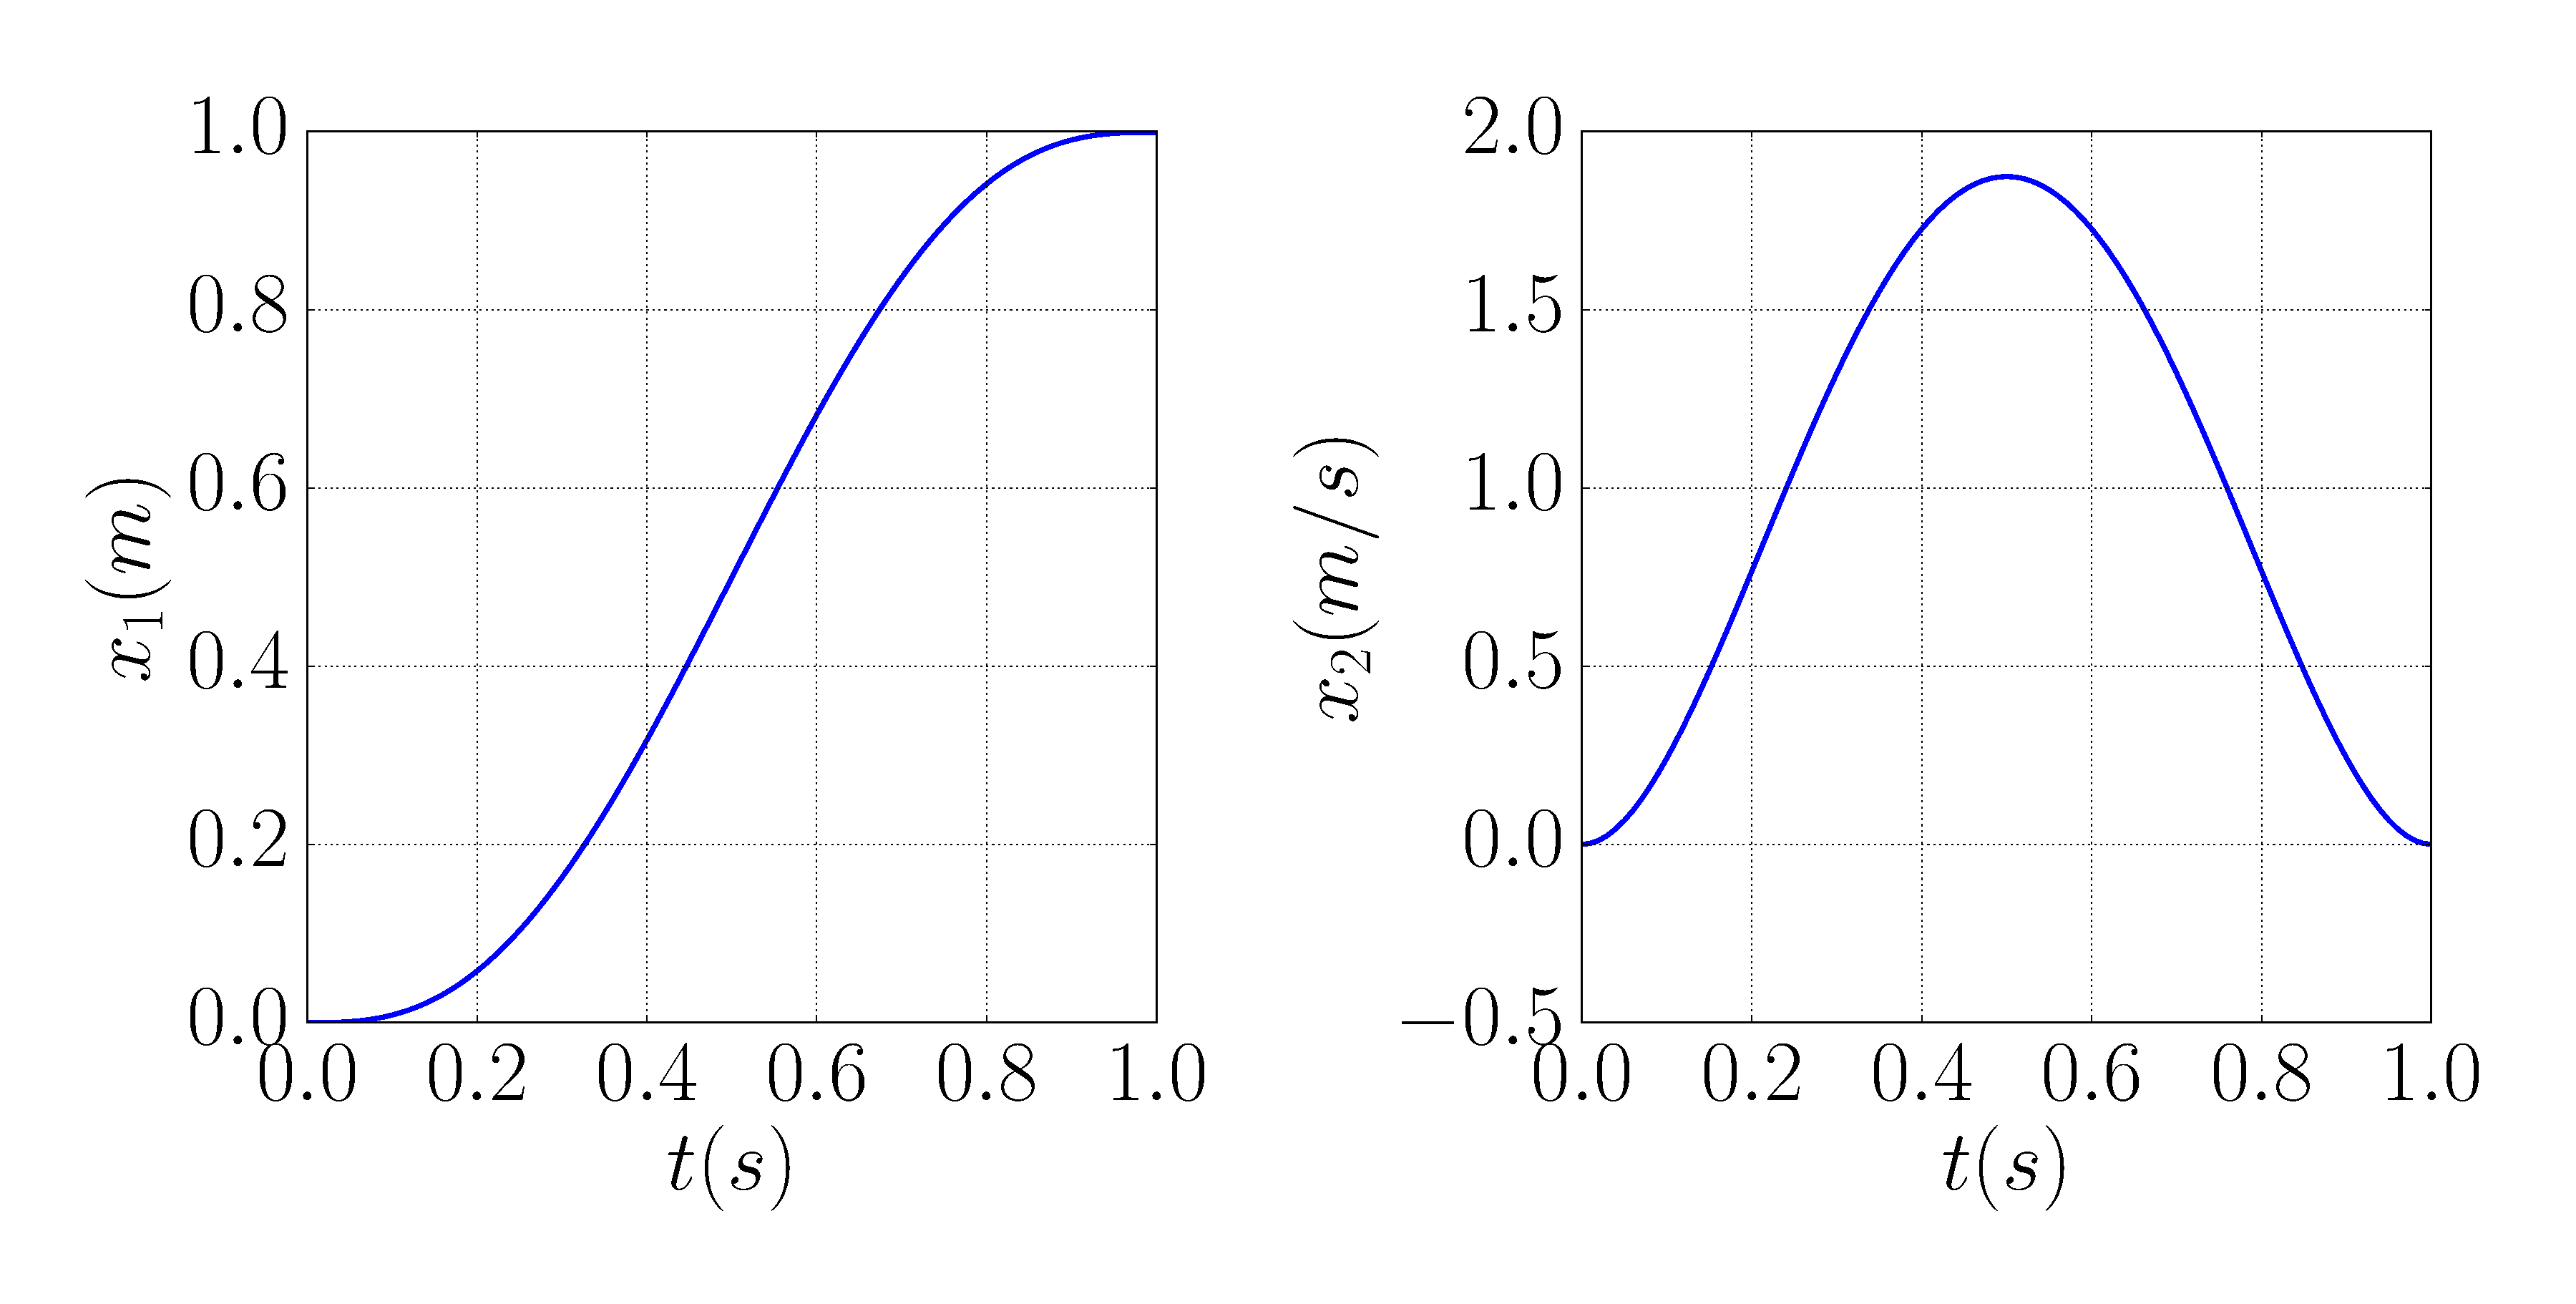
\includegraphics[width=15.5cm]{bild/30_32/test0_ohne_k_ori_x.pdf}
		\caption{Verlauf der Systemzustände vom System ohne der Wirkung von k. $x_{1}$ und $x_{2}$ steht für Position und Geschwindigkeit.}
		\label{fig:Doppelintegrator_ohne_k_x}
	\end{figure}
	
	
	
	\begin{figure}
		\centering
		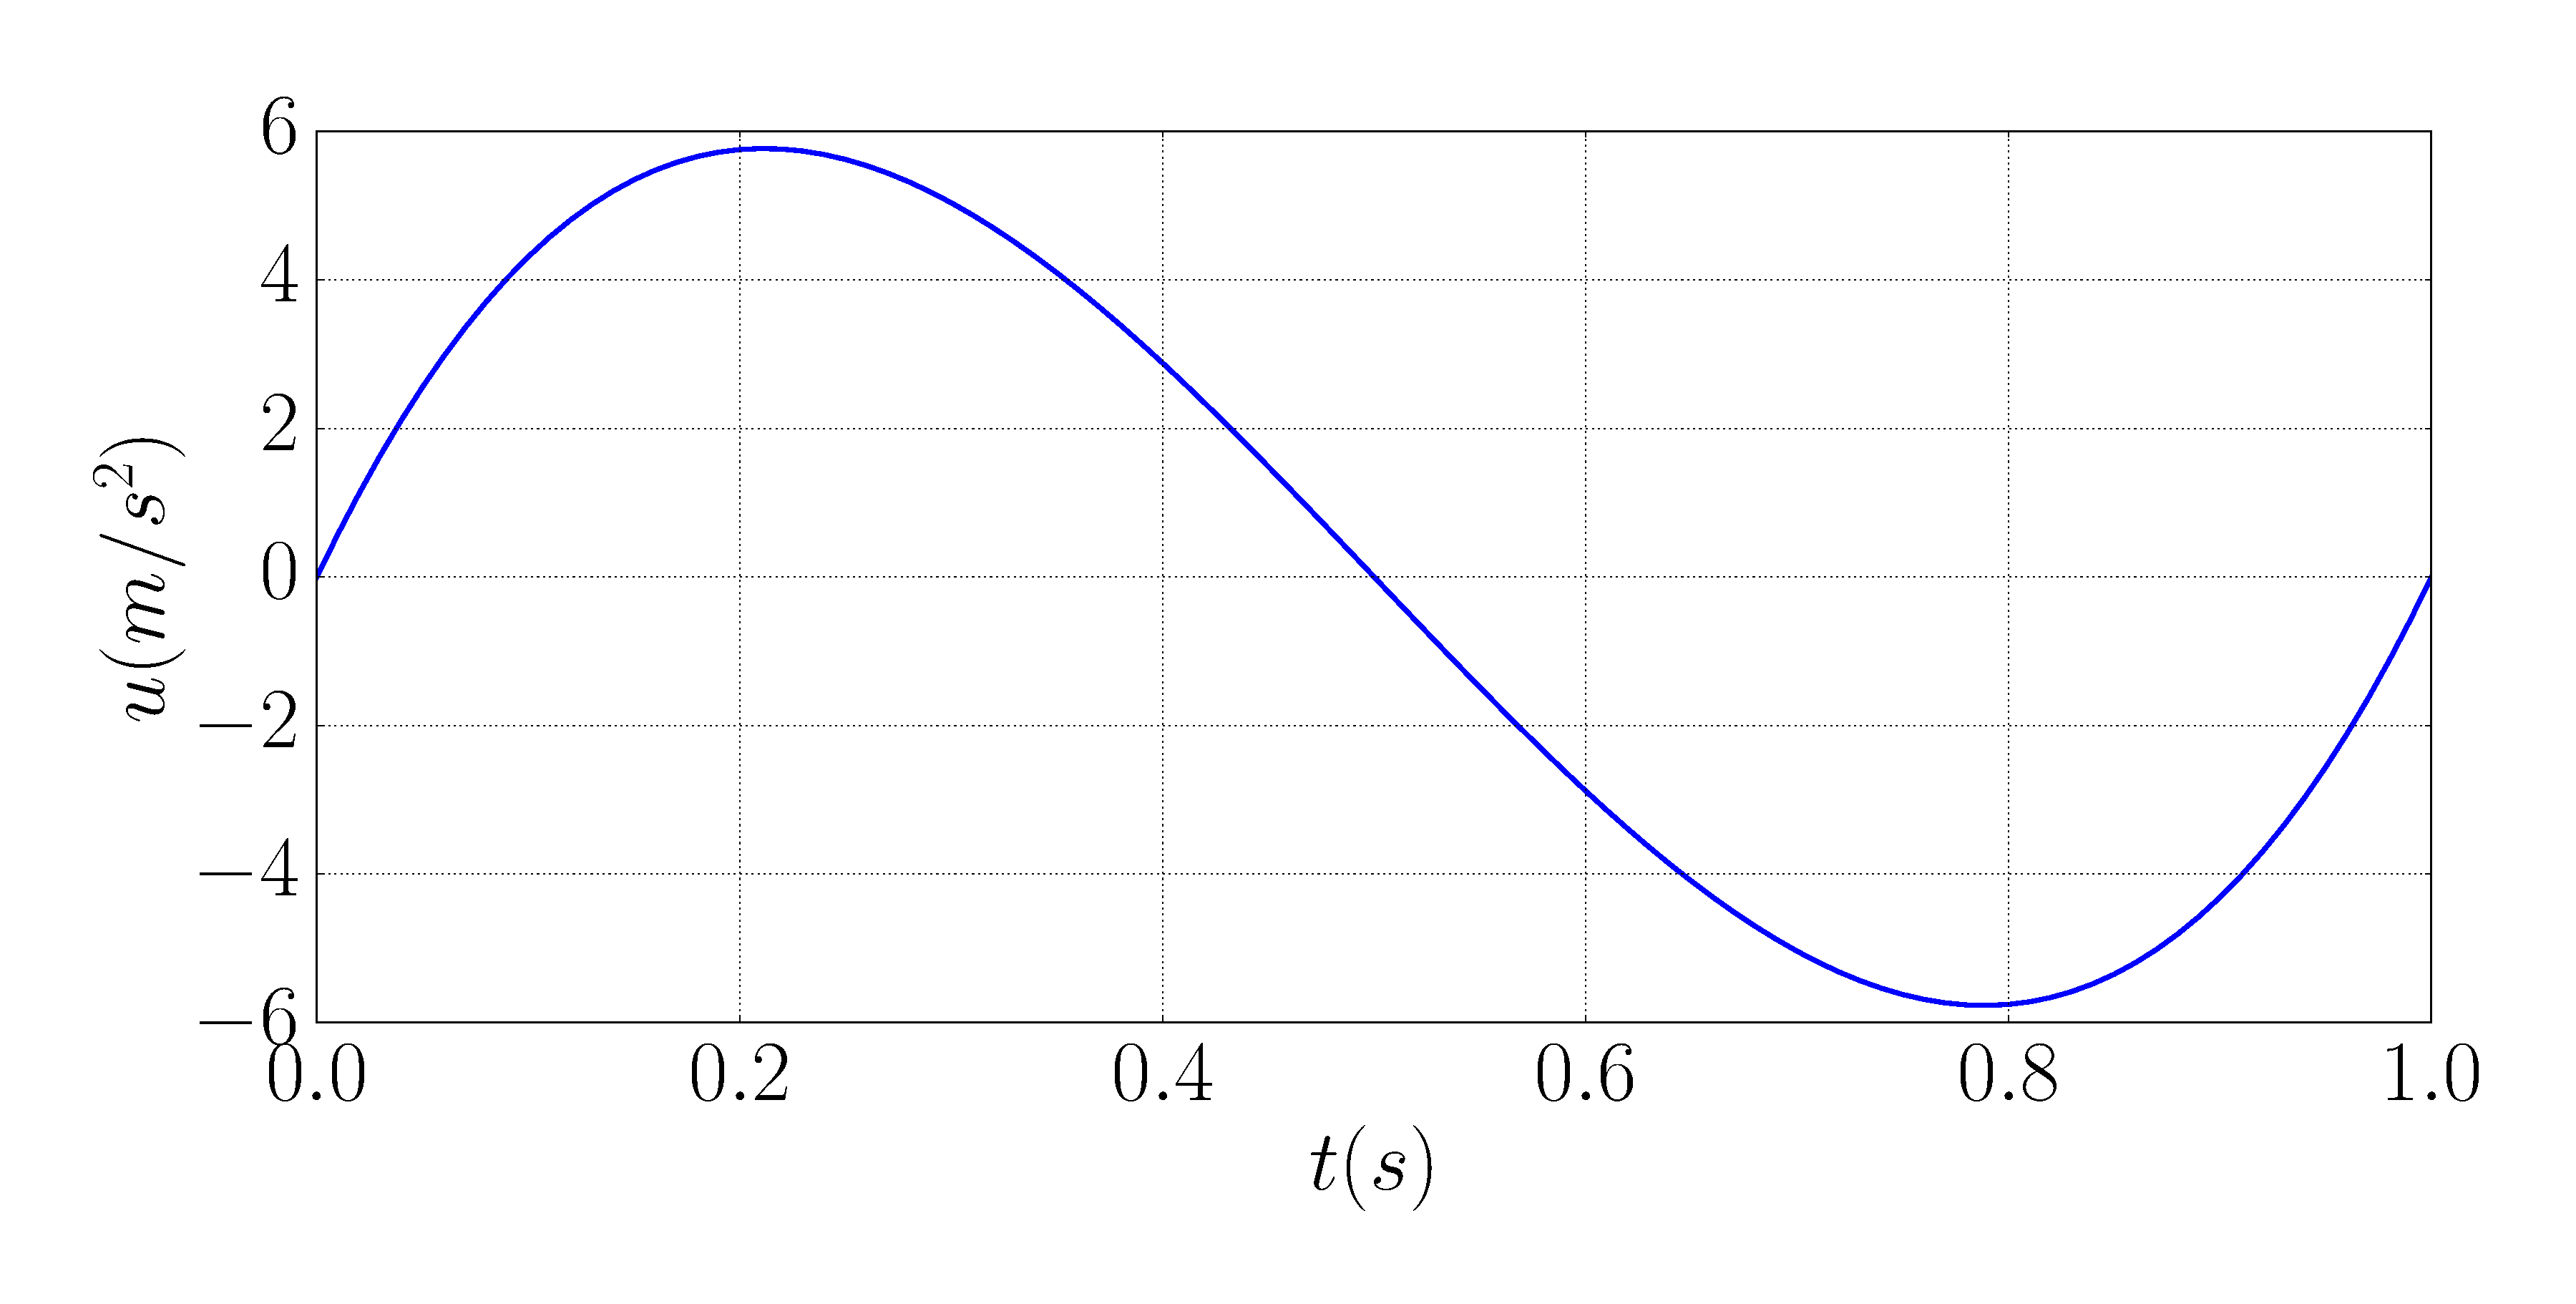
\includegraphics[width=12cm]{bild/30_32/test0_ohne_k_ori_u.pdf}
		\caption{Verlauf des Systemeingangs vom System ohne der Wirkung von k. $u_{1}$ steht für Waagebeschleunigung.}
		\label{fig:Doppelintegrator_ohne_k_u}
	\end{figure}
	
	Andererseits ist die Trajektorie für das System mit ``k''. Aus Abb. \ref{fig:Doppelintegrator_mit_k_x} und Abb. \ref{fig:Doppelintegrator_mit_k_u} beobachtet man darauf, zwar die maximale Kraft und die Geschwindigkeit weit kleiner als die im oberen System, ist der Wert von $k$ hier ziemlich groß (ungefähr $1662,53s$)! Der Wagen in diesem System muss $1662s$ lang bewegen, bevor er die Endposition angekommen. Daher ist die Lösung von $k$ \textbf{richtig} aber \textbf{nicht rational}.
	\begin{figure}
		\centering
		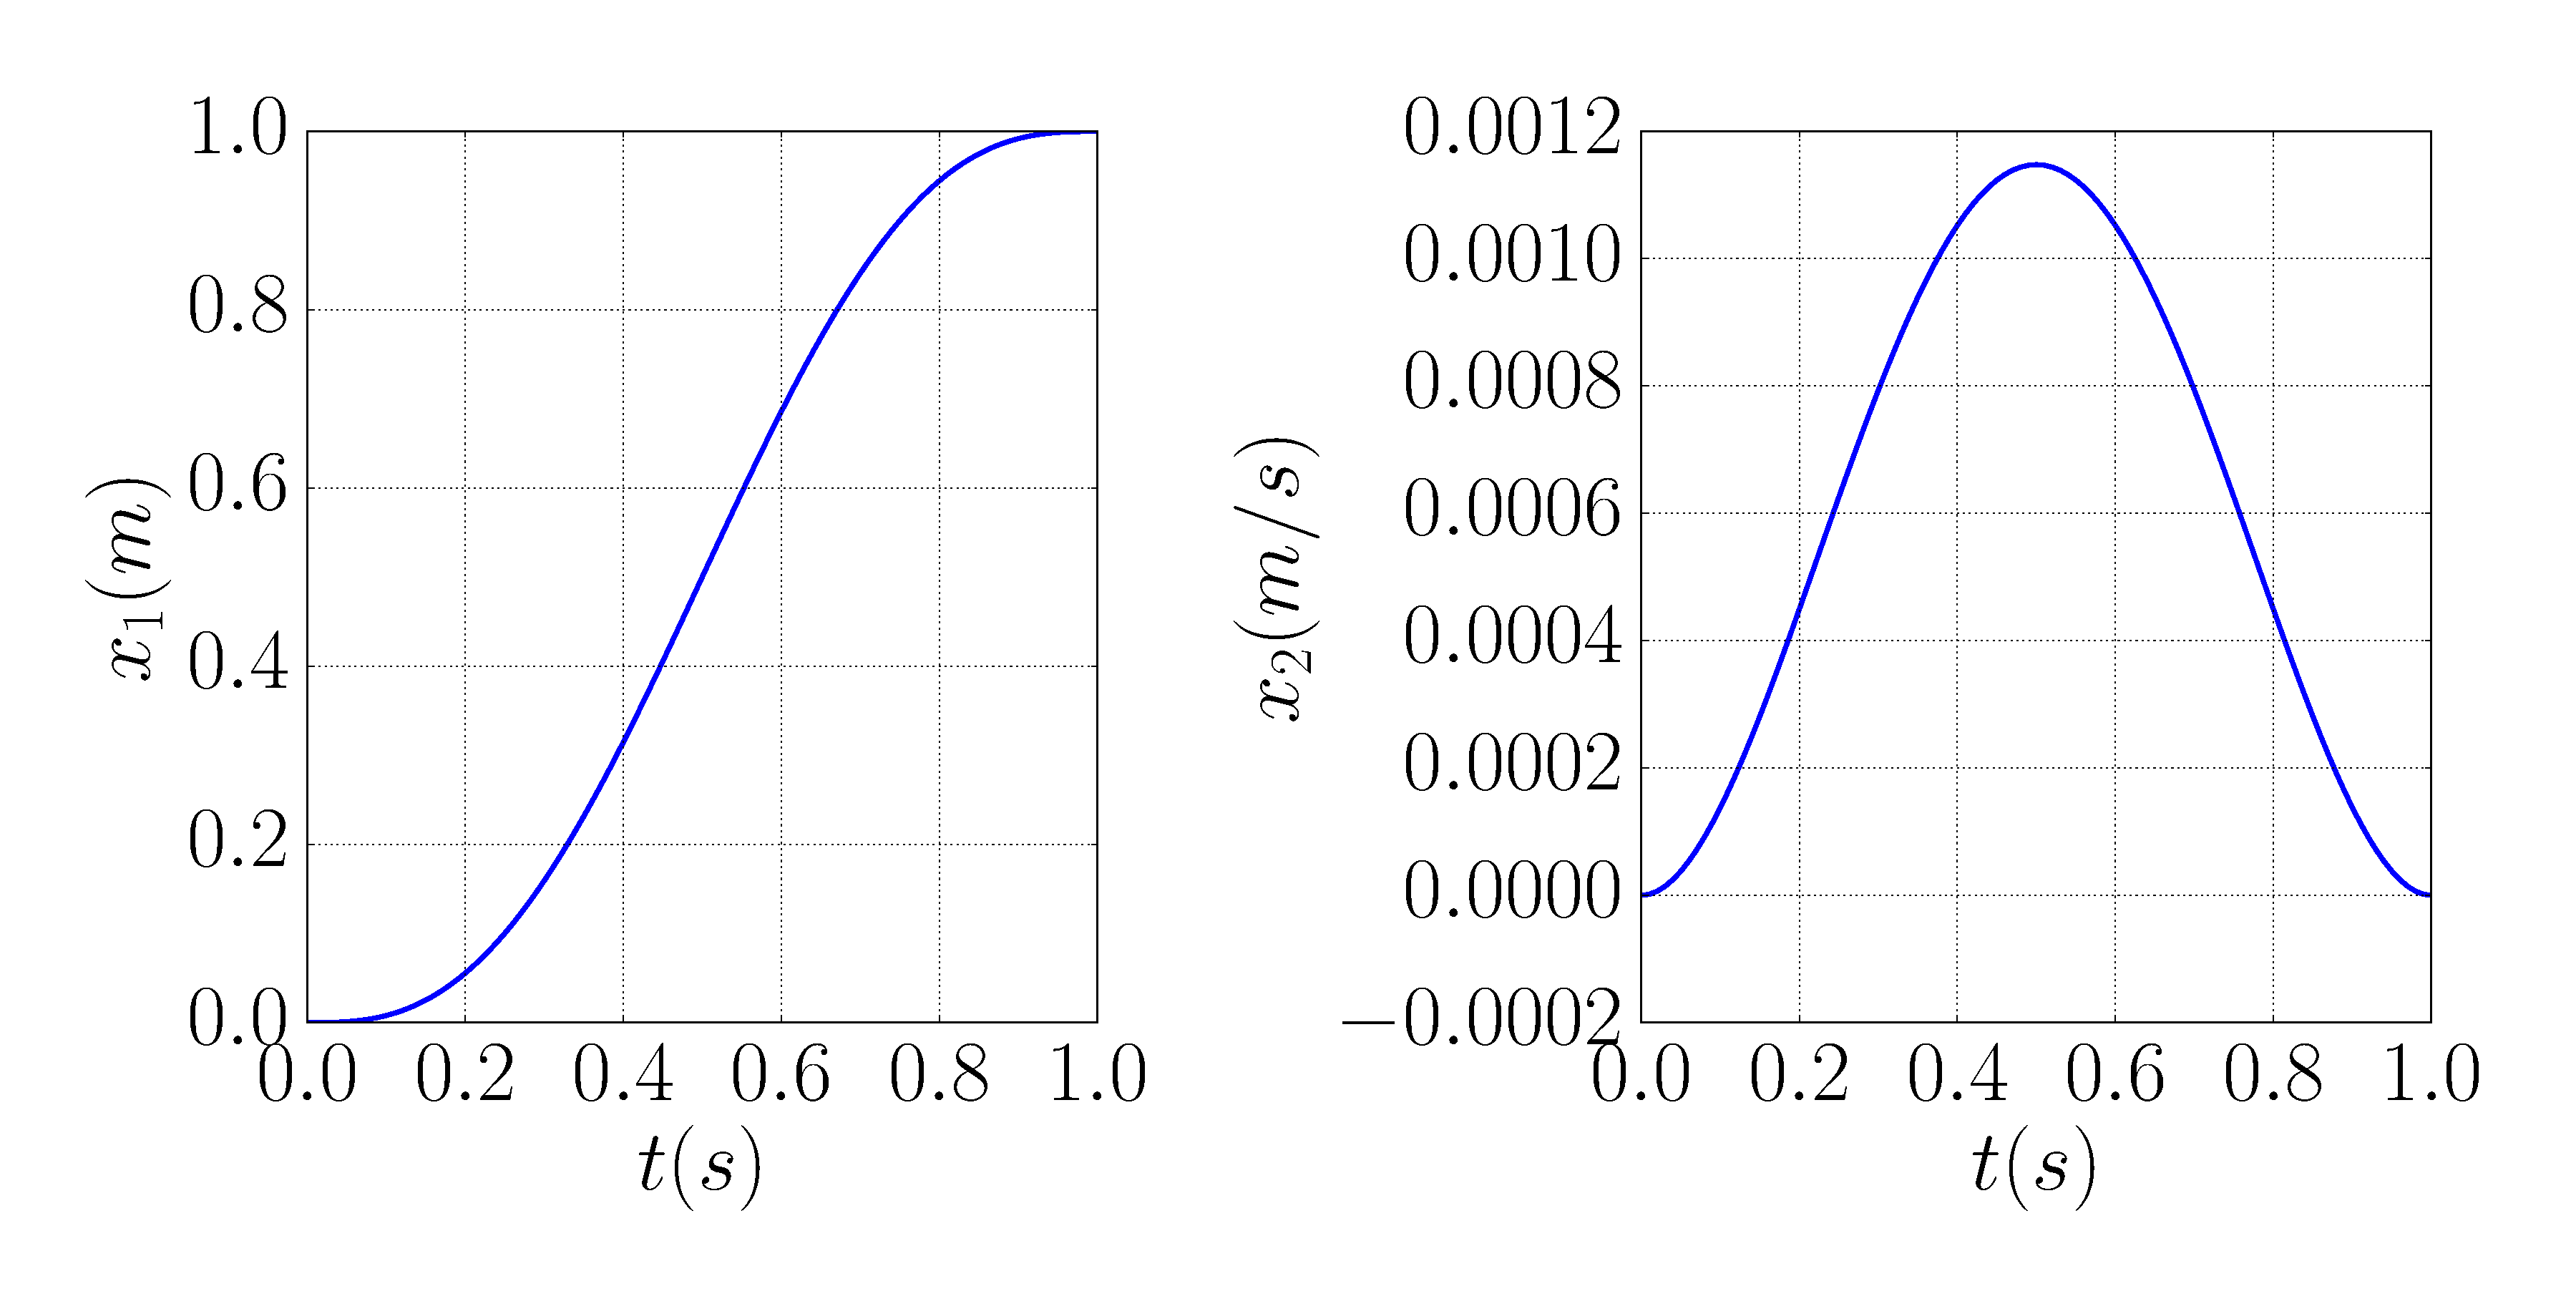
\includegraphics[width=15.5cm]{bild/30_32/test0_mit_k_ori_x.pdf}
		\caption{Verlauf des Systemeingangs vom System mit der Wirkung von k. $u_{1}$ steht für Wagenbeschleunigung.}
		\label{fig:Doppelintegrator_mit_k_x}
	\end{figure}
	\begin{figure}
		\centering
		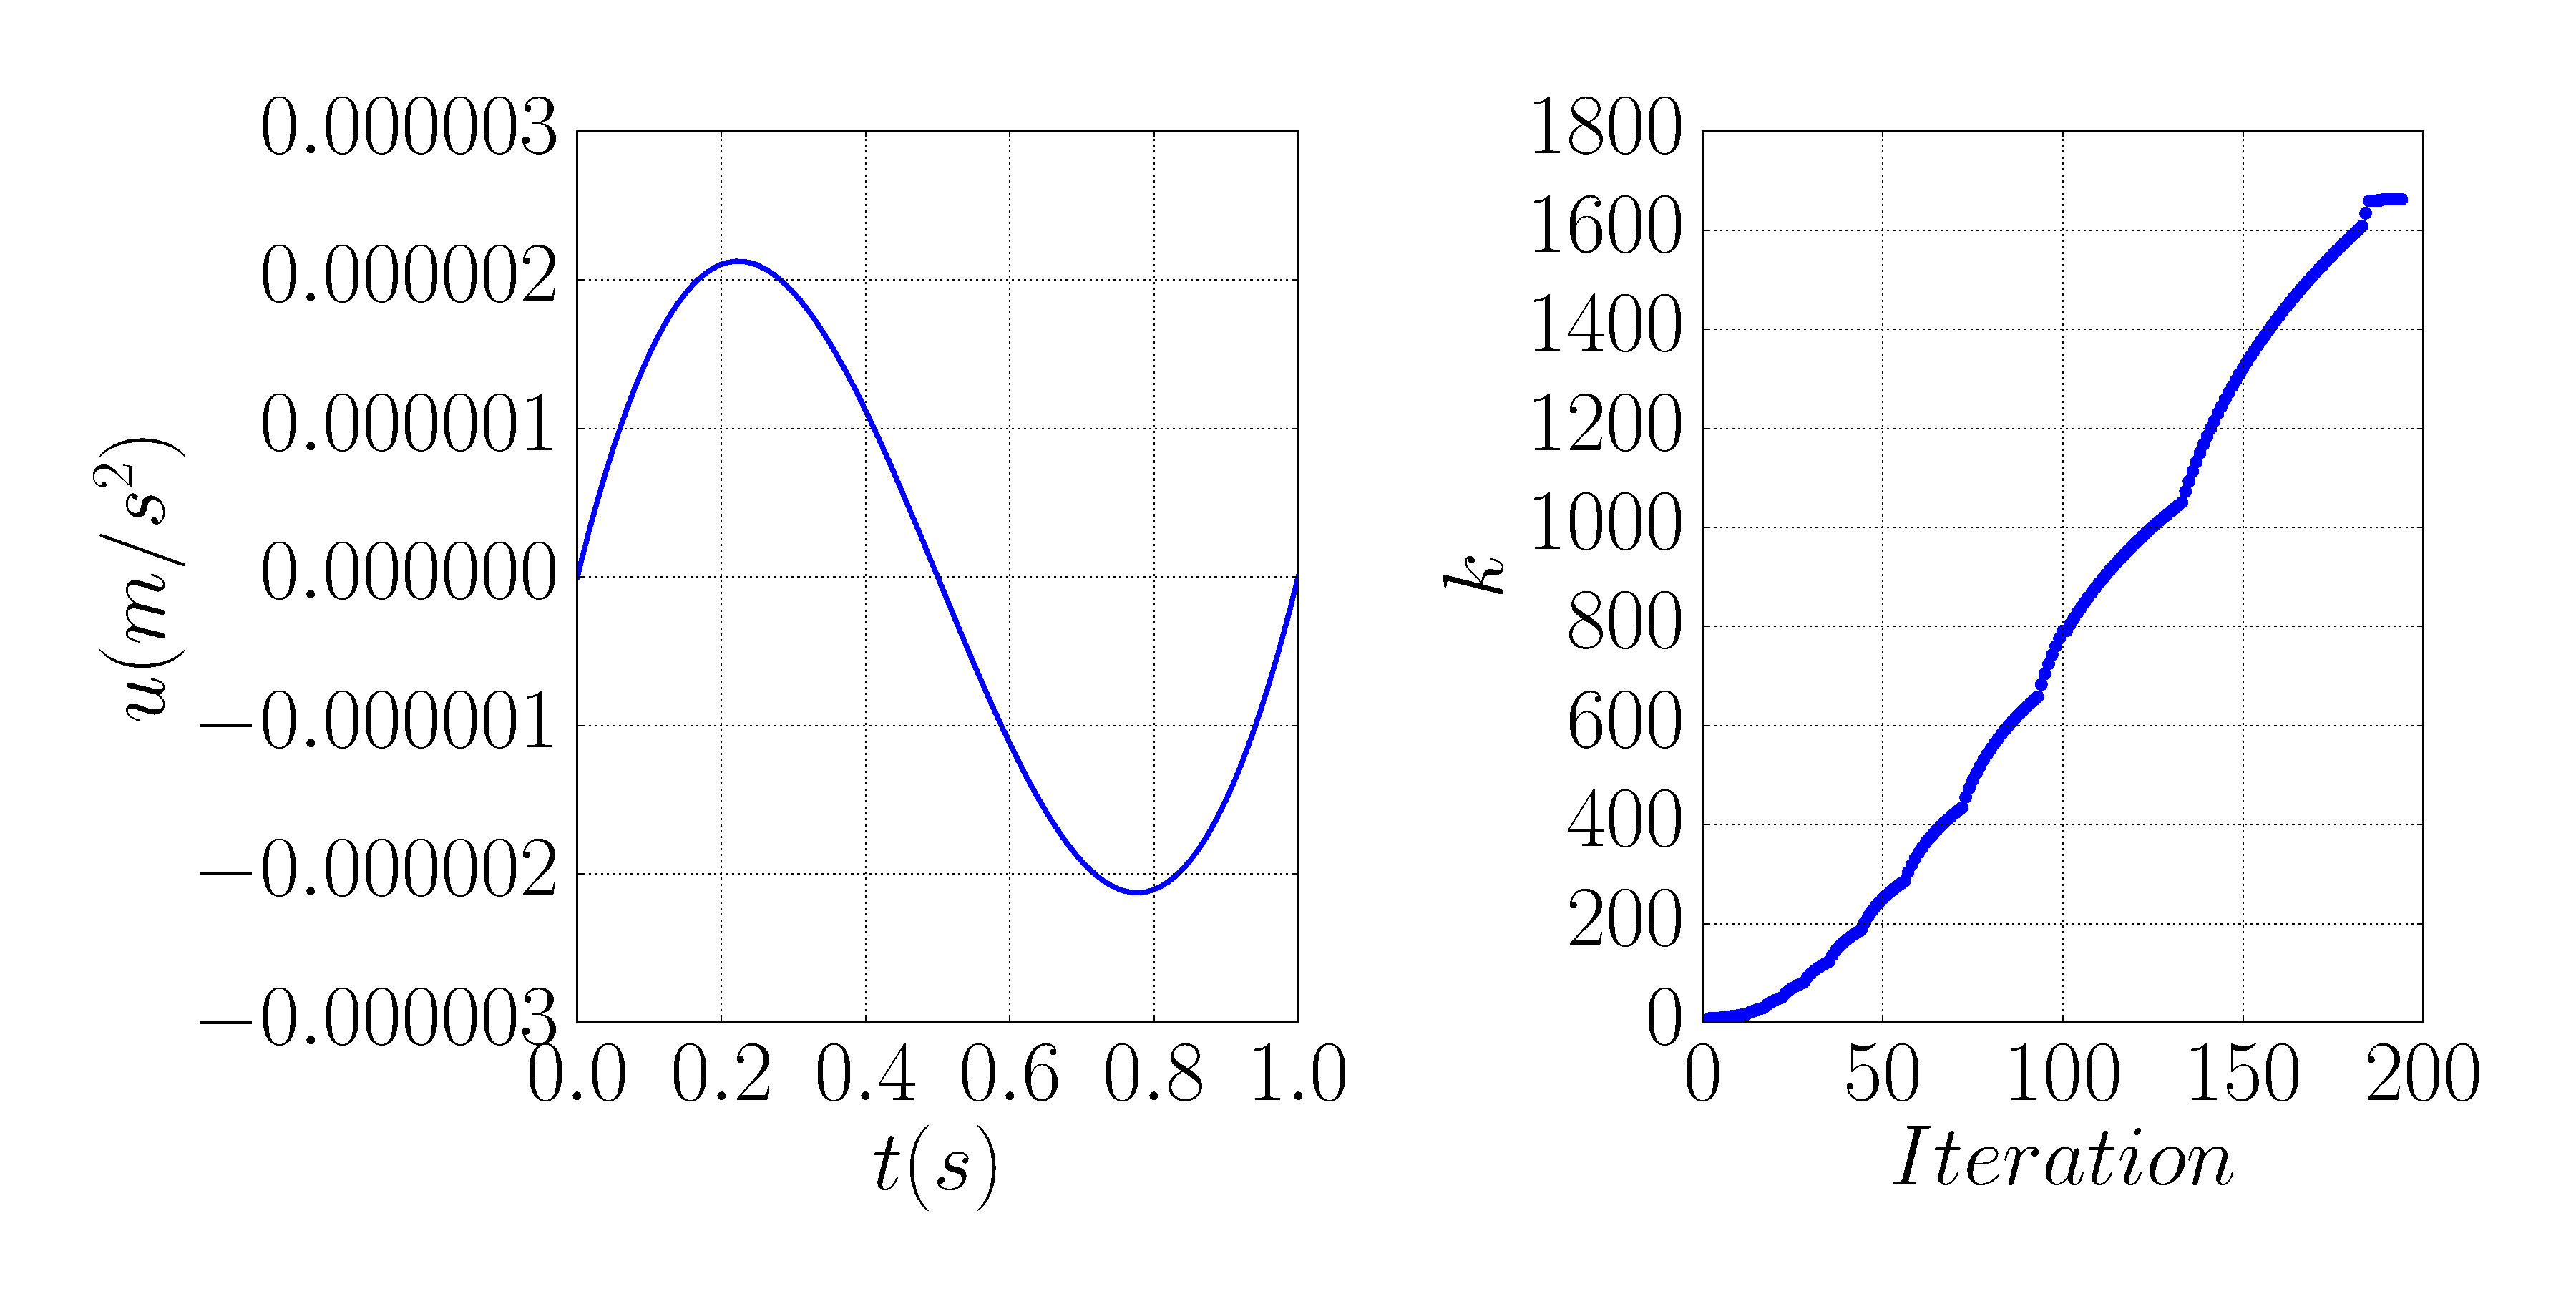
\includegraphics[width=12cm]{bild/30_32/test0_mit_k_ori_u.pdf}
		\caption{Verlauf der Systemzustände vom System mit der Wirkung von k. $x_{1}$ und $x_{2}$ steht für Position und Geschwindigkeit.}
		\label{fig:Doppelintegrator_mit_k_u}
	\end{figure}
	
	Zur Verbesserung des Ergebnisses wird eine andere Anfangswert der Polynomparameter gewählt. Statt aller Werte $0.1$ sind die Parameter jetzt gleich die Rechenergebnisse von Polynomparameter nach der ersten Iteration in dem System ohne ``k''. Die Kurven in Abb. \ref{fig:Doppelintegrator_mit_k_x_aus} und \ref{fig:Doppelintegrator_mit_k_u_aus} sehen ähnlich wie Abb. \ref{fig:Doppelintegrator_ohne_k_x} und Abb.  \ref{fig:Doppelintegrator_ohne_k_u} mit einem kleinen $k=1.21$. Endlich stoppt der Wagen in $1.21$s am $1$m. 
	\begin{figure}
		\centering
		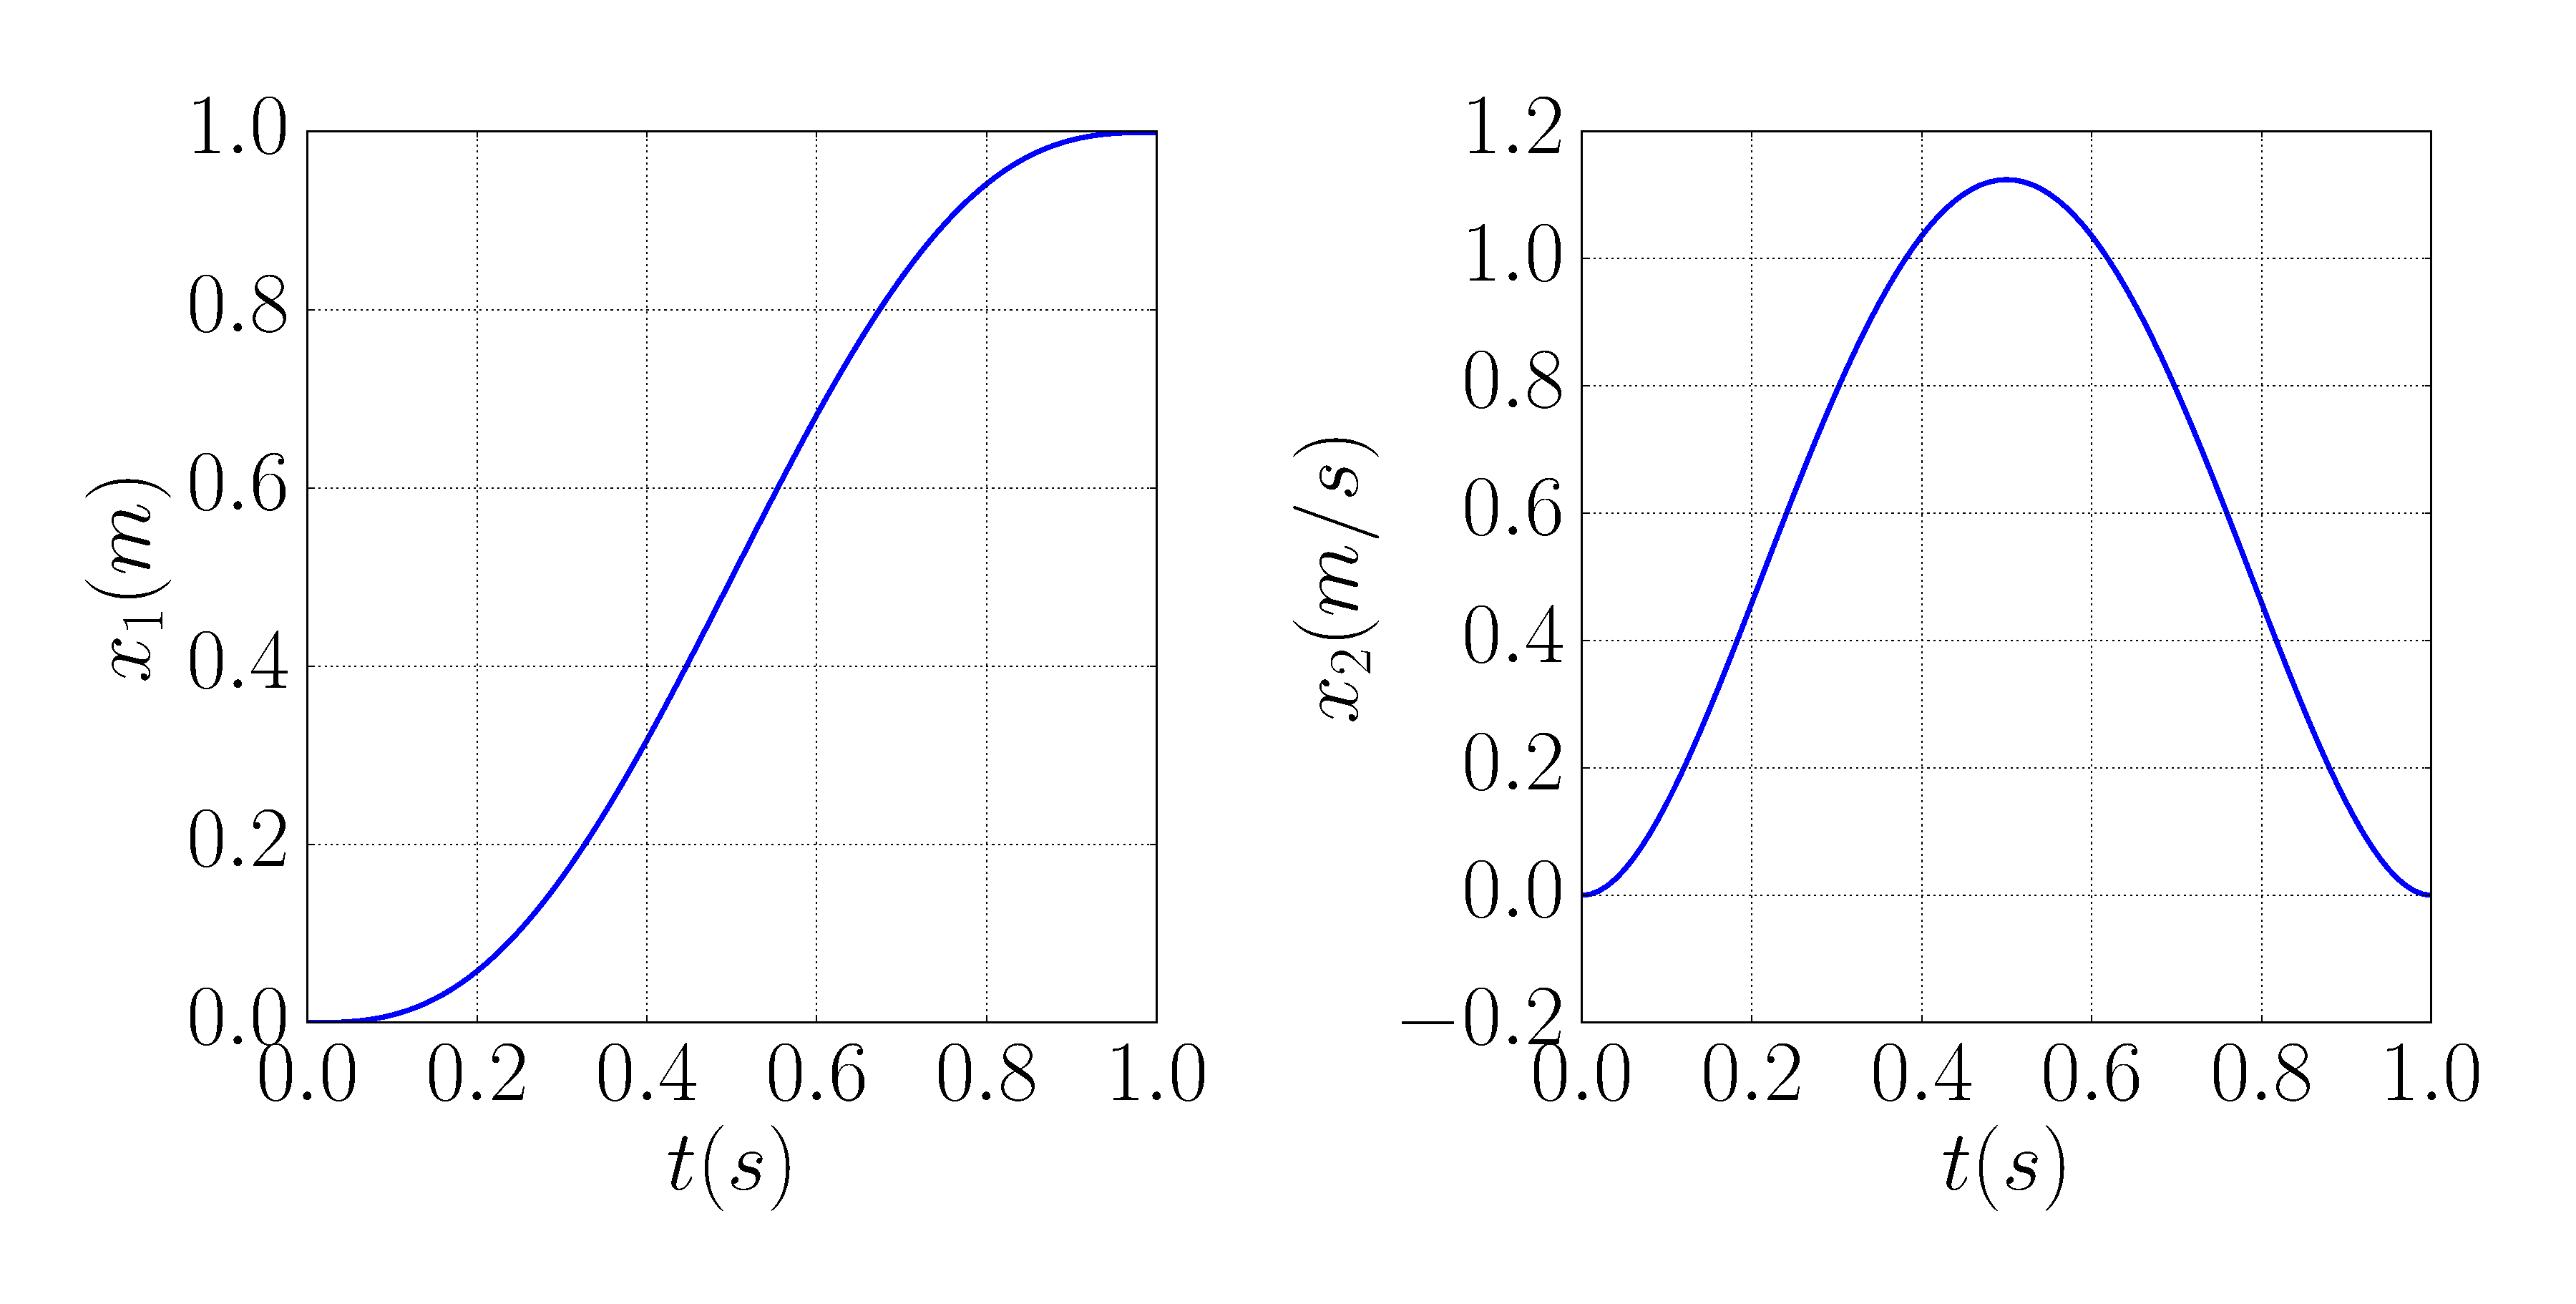
\includegraphics[width=15.5cm]{bild/30_32/test0_mit_k_Ite1_x.pdf}
		\caption{Verlauf des Systemeingangs vom System mit der Wirkung von k. $u_{1}$ steht für Waagebeschleunigung.}
		\label{fig:Doppelintegrator_mit_k_x_aus}
	\end{figure}

	\begin{figure}
		\centering
		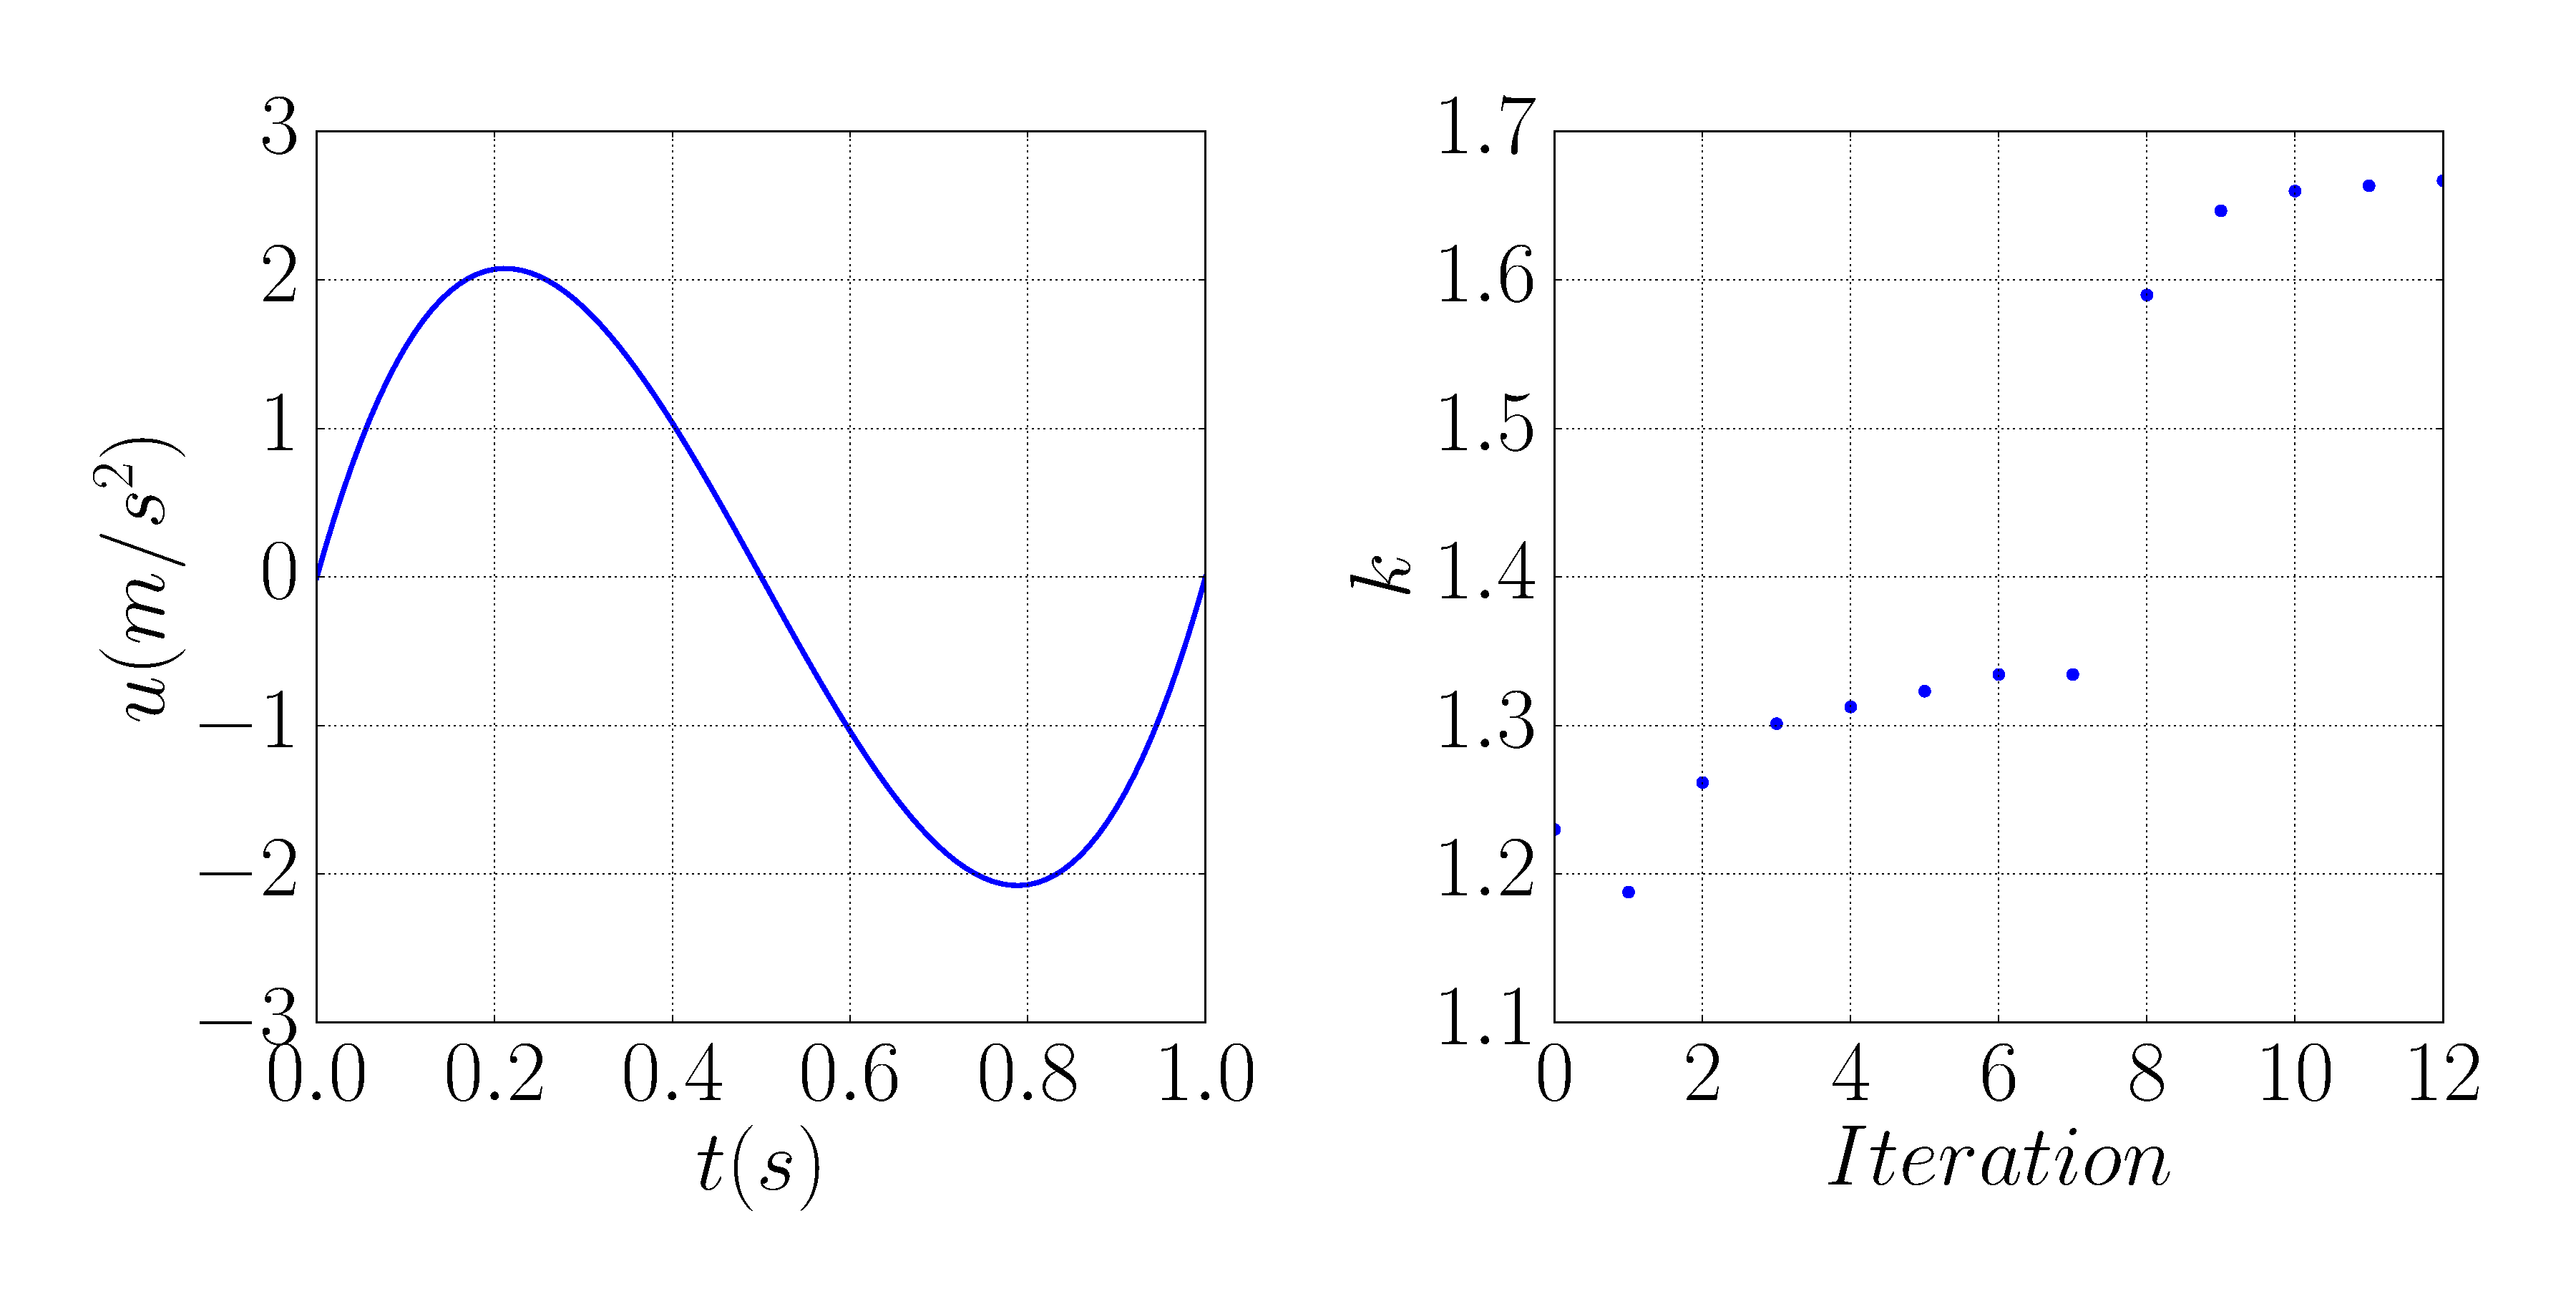
\includegraphics[width=12cm]{bild/30_32/test0_mit_k_Ite1_u.pdf}
		\caption{Verlauf des Systemeingangs vom System mit der Wirkung von k. $u_{1}$ steht für Waagebeschleunigung.}
		\label{fig:Doppelintegrator_mit_k_u_aus}
	\end{figure}
	
\end{beispiel}
\newpage
Dieses Beispiel zeigt die starke Abhängigkeit der Konvergenzmöglichkeit von Levenberg-Marquadt-Algorithmus und des Anfangsschätzwerts. Wenn die Anfangsschätzwerte der Parameter zu weit vom Minimierer eingestellt sind, kann die Methode das System nicht konvergiert oder zu einem lokalen, nicht globalen optimierten Punkt richten.

Das folgende Beispiel stellt die Anwendung der LM-Methode in einem verbreiterten Benchmark System vor.

\begin{beispiel}[System–Inverses-Pendel]
	Abb. \ref{fig:Inverses-Pendel} zeigt das Schema des inversen Pendels. Der Pendelarm ist auf einem horizontal bewegten Wagen montiert. Der Wagen bringt daher eine horizontale Kraft auf das Pendel auf. Beim Aufprägen der Kraft $\vec{F}$ auf den Wagen bewegt sich das Pendel von oben nach unten. Die instabile Ruhelage ist der Punkt, in dem das Pendel genau senkrecht zum Wagen steht und der Drehwinkel $180^{\circ}$ beträgt. Systemvariable in diesem Modell sind die Wagenposition $\vect{x}_{1}$, dessen Geschwindigkeit $\vect{x}_{2}$, der Pendeldrehwinkel $\vect{x}_{3}$, die Drehgeschwindigkeit davon $\vect{x}_{4}$. Der einzige Systemeingang ist die auf den Wagen aufgeprägte Kraft $f_{w}$.
	\begin{figure}
		\centering
		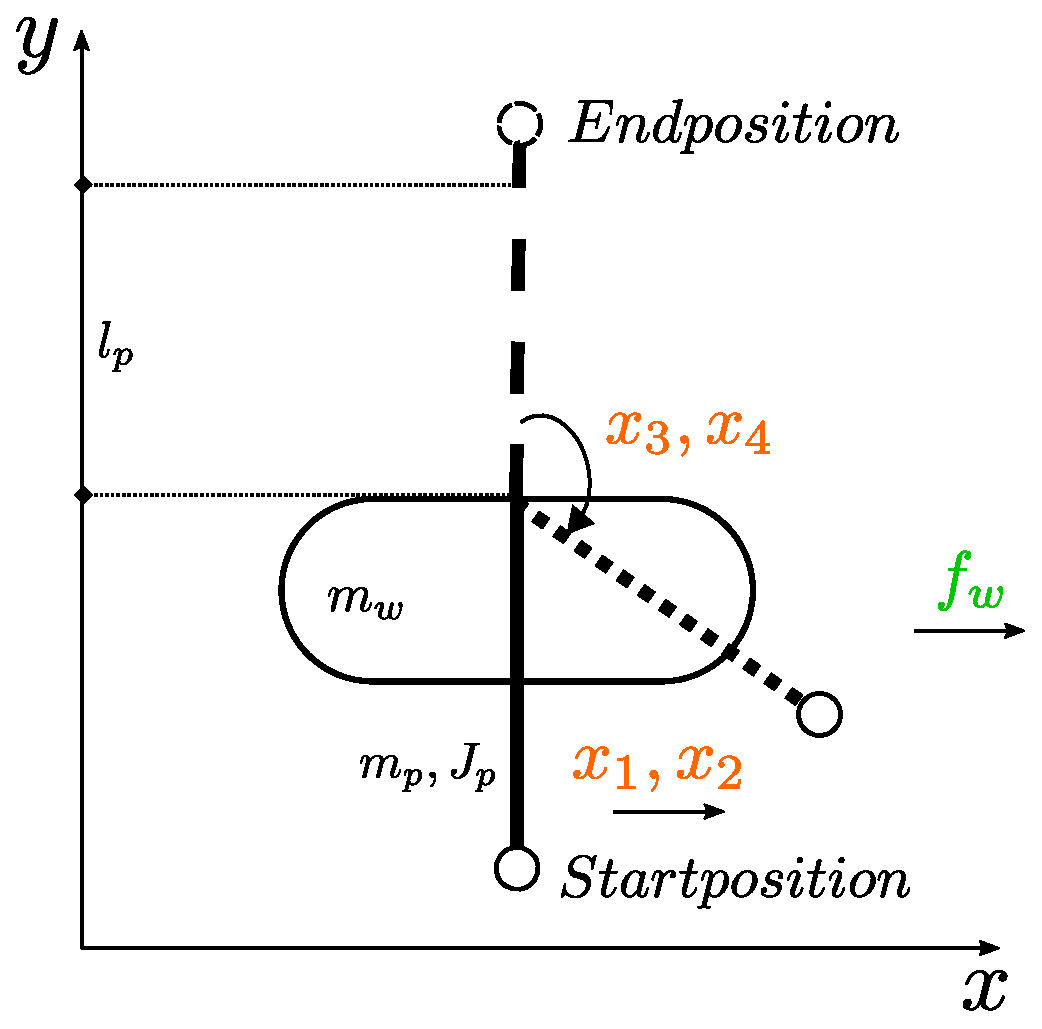
\includegraphics[width=6cm]{bild/modul/Inverses-Pendel.eps}
		\caption{Struktur des inversen Pendels: in dem System gibt es vier Zustände $\vec{x}_{1}$ bis $\vec{x}_{4}$. Das Pendel folgt einer gegebenen Trajektorie und bewegt sich von $180^{\circ}$ bis zur instabilen Ruhelage (nämlich vom ganz unten zu ganz oben). $m_{w}$ und $m_{p}$ sind jeweils die Masse des Wagens und des Pendels, $J_{p}$ ist das Trägheitsmoment und $l_{p}$ ist der Abstand zwischen dem Stützpunkt und dem Pendelschwerpunkt. Die Pfeile neben Zuständen geben die Vektorrichtung an.}
		\label{fig:Inverses-Pendel}
	\end{figure}  

	Dazugehörende Differentialgleichungen des Modells sind wie folgt beschrieben\cite{TUM}\cite{MAMoh}:
	\begin{eqnarray}
	\dot{x}_{1}&=&x_{2}\notag\\
	\dot{x}_{2}&=&\frac{\left ( J_{p}+m_{p}{l_{p}}^{2} \right )\left ( -f_{w}x_{2}+m_{p}l_{p}sin(x_{3})x_{4}^{2}+x_{5}\right )+m_{p}l_{p}f_{p}cos(x_{3})x_{4}}{\left ( m_{w}+m_{p} \right )J_{p}+m_{w}m_{p}{l_{p}}^{2}+{m_{p}}^{2}{l_{p}}^{2}sin^{2}(x_{3})}\notag\\&+&\frac{m_{p}l_{p}f_{p}cos(x_{3})z_{4}+{m_{p}}^{2}{l_{p}}^{2}gcos(x_{3})sin(x_{4})}{\left ( m_{w}+m_{p} \right )J_{p}+m_{w}m_{p}{l_{p}}^{2}+{m_{p}}^{2}{l_{p}}^{2}sin^{2}(x_{3})}\notag
	\\
	\dot{x}_{3}&=&x_{4}\notag\\
	\dot{x}_{4}&=&\frac{-m_{p}l_{p}cos(x_{3})x_{5}+f_{w}m_{p}l_{p}cos(x_{3})x_{2}- {m_{p}}^{2}{l_{p}}^{2}cos(x_{3})sin(x_{3})x_{4}^{2}}{\left ( m_{w}+m_{p} \right )J_{p}+m_{w}m_{p}{l_{p}}^{2}+{m_{p}}^{2}{l_{p}}^{2}sin(x_{3}^{2})}\notag\\&-&\frac{\left ( m_{w}+m_{p} \right )f_{w}x_{4}+\left ( m_{w}+m_{p} \right )gm_{p}l_{p}sin(x_{3})}{\left ( m_{w}+m_{p} \right )J_{p}+m_{w}m_{p}{l_{p}}^{2}+{m_{p}}^{2}{l_{p}}^{2}sin(x_{3}^{2})}\label{eq:DLG_Inverses_Pendel}  
	\end{eqnarray}
	
	Vereinfachen die Gleichungen und Ignorieren kleiner Teiler erhält man eine kompakte Zustandsdarstellung des inversen Pendels\cite{kunze2016pytrajectory}:
	\begin{eqnarray}
	\dot{x}_{1}&=&x_{2}\notag\\
	\dot{x}_{2}&=&\frac{m_{p}sin(x_{3})(-l_{p}x_{4}^{2}+gcos(x_{3}))}{m_{w}l_{p}+m_{p}sin^{2}(x_{3})}+\frac{cos(x_{3})}{m_{w}l_{p}+m_{p}l_{p}sin^{2}(x_{3})}u\notag\\
	\dot{x}_{3}&=&x_{4}\notag\\
	\dot{x}_{4}&=&\frac{sin(x_{3})(-m_{p}l_{p}x_{4}^{2}cos(x_{3})+g(m_{w}+m_{p}))}{m_{w}l_{p}+m_{p}sin^{2}(x_{3})}+\frac{cos(x_{3})}{m_{w}l_{p}+m_{p}sin^{2}(x_{3})}u\label{eq:DLG_Inverses_Pendel_compact}   
	\end{eqnarray}
	
	Wenn das System partiell linearisiert und einen virtuellen Eingang, die Beschleunigung des Wagens $\dot{x}_{2}$ anstatt der Kraft $u$ gegeben wird, lässt sich die Systemdarstellung vielmehr einfacher darstellen:
	\begin{eqnarray}
	\dot{x}_{1}&=&x_{2}\notag\\
	\dot{x}_{2}&=&u\notag\\
	\dot{x}_{3}&=&x_{4}\notag\\
	\dot{x}_{4}&=&\frac{g}{l_{p}}sin(x_{3})+\frac{1}{l_{p}}cos(x_{3})u\label{eq:DLG_Inverses_Pendel_partiell_lin}   
	\end{eqnarray}
	
	Weil der Pendel sich von unten nach oben drehen und der Wagen endlich zum Startpunkt zurückgehen soll, ist die Trajektorie wie $\left ( 0,0,\pi ,0 \right )\rightarrow \left ( 0,0,0,0 \right )$ erfordert. Der Anfangszahl der Spline-Abschnitt und das Iterationsvielfache ist jeweils $2$. All die Anfangsschätzwerte der Polynomkoeffizienten sind $0.1$. Die Ergebnisse sind in Abb. \ref{fig:Inverses_Pendel_ohne_k_x}, Abb. \ref{fig:Inverses_Pendel_ohne_k_u}, Abb. \ref{fig:Inverses_Pendel_mit_k_x_ori} und Abb. \ref{fig:Inverses_Pendel_mit_k_u_ori} dargestellt.
	
	\begin{figure}
		\centering
		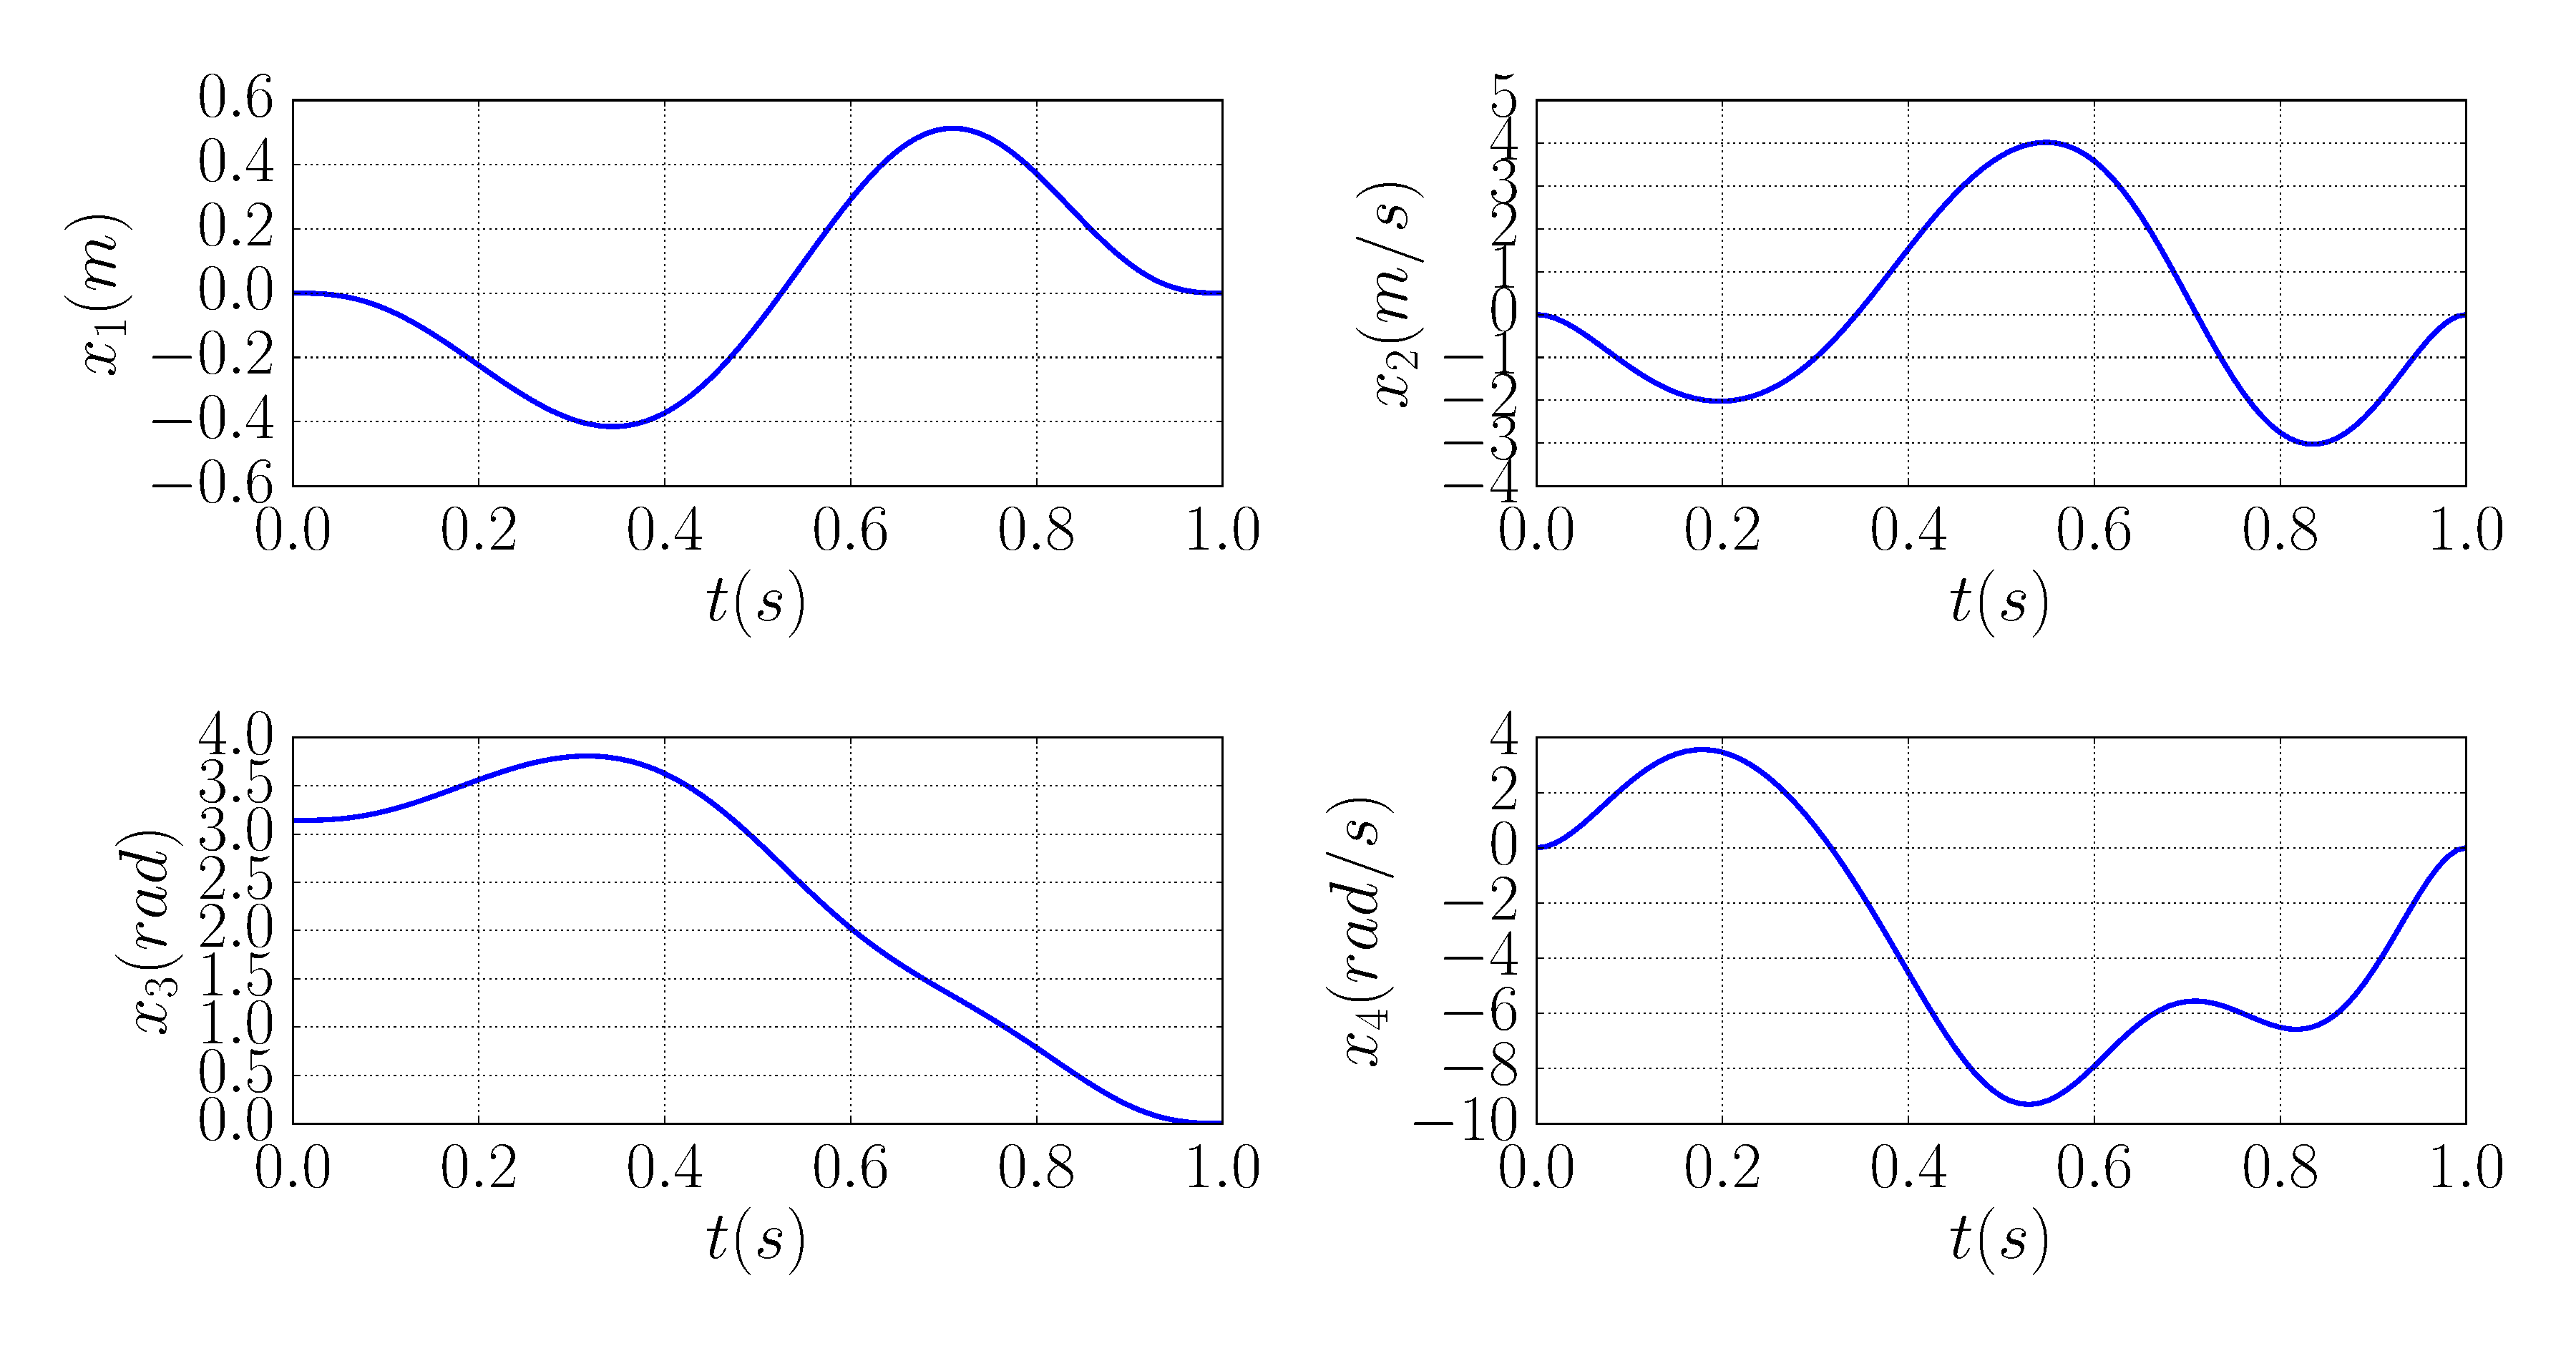
\includegraphics[width=15.5cm]{bild/30_32/example0_ohne_k_x.pdf}
		\caption{Systemzuständen des inversen-Pendels (ohne k) mit dem virtuellen Eingang.}
		\label{fig:Inverses_Pendel_ohne_k_x}
	\end{figure}

	\begin{figure}
		\centering
		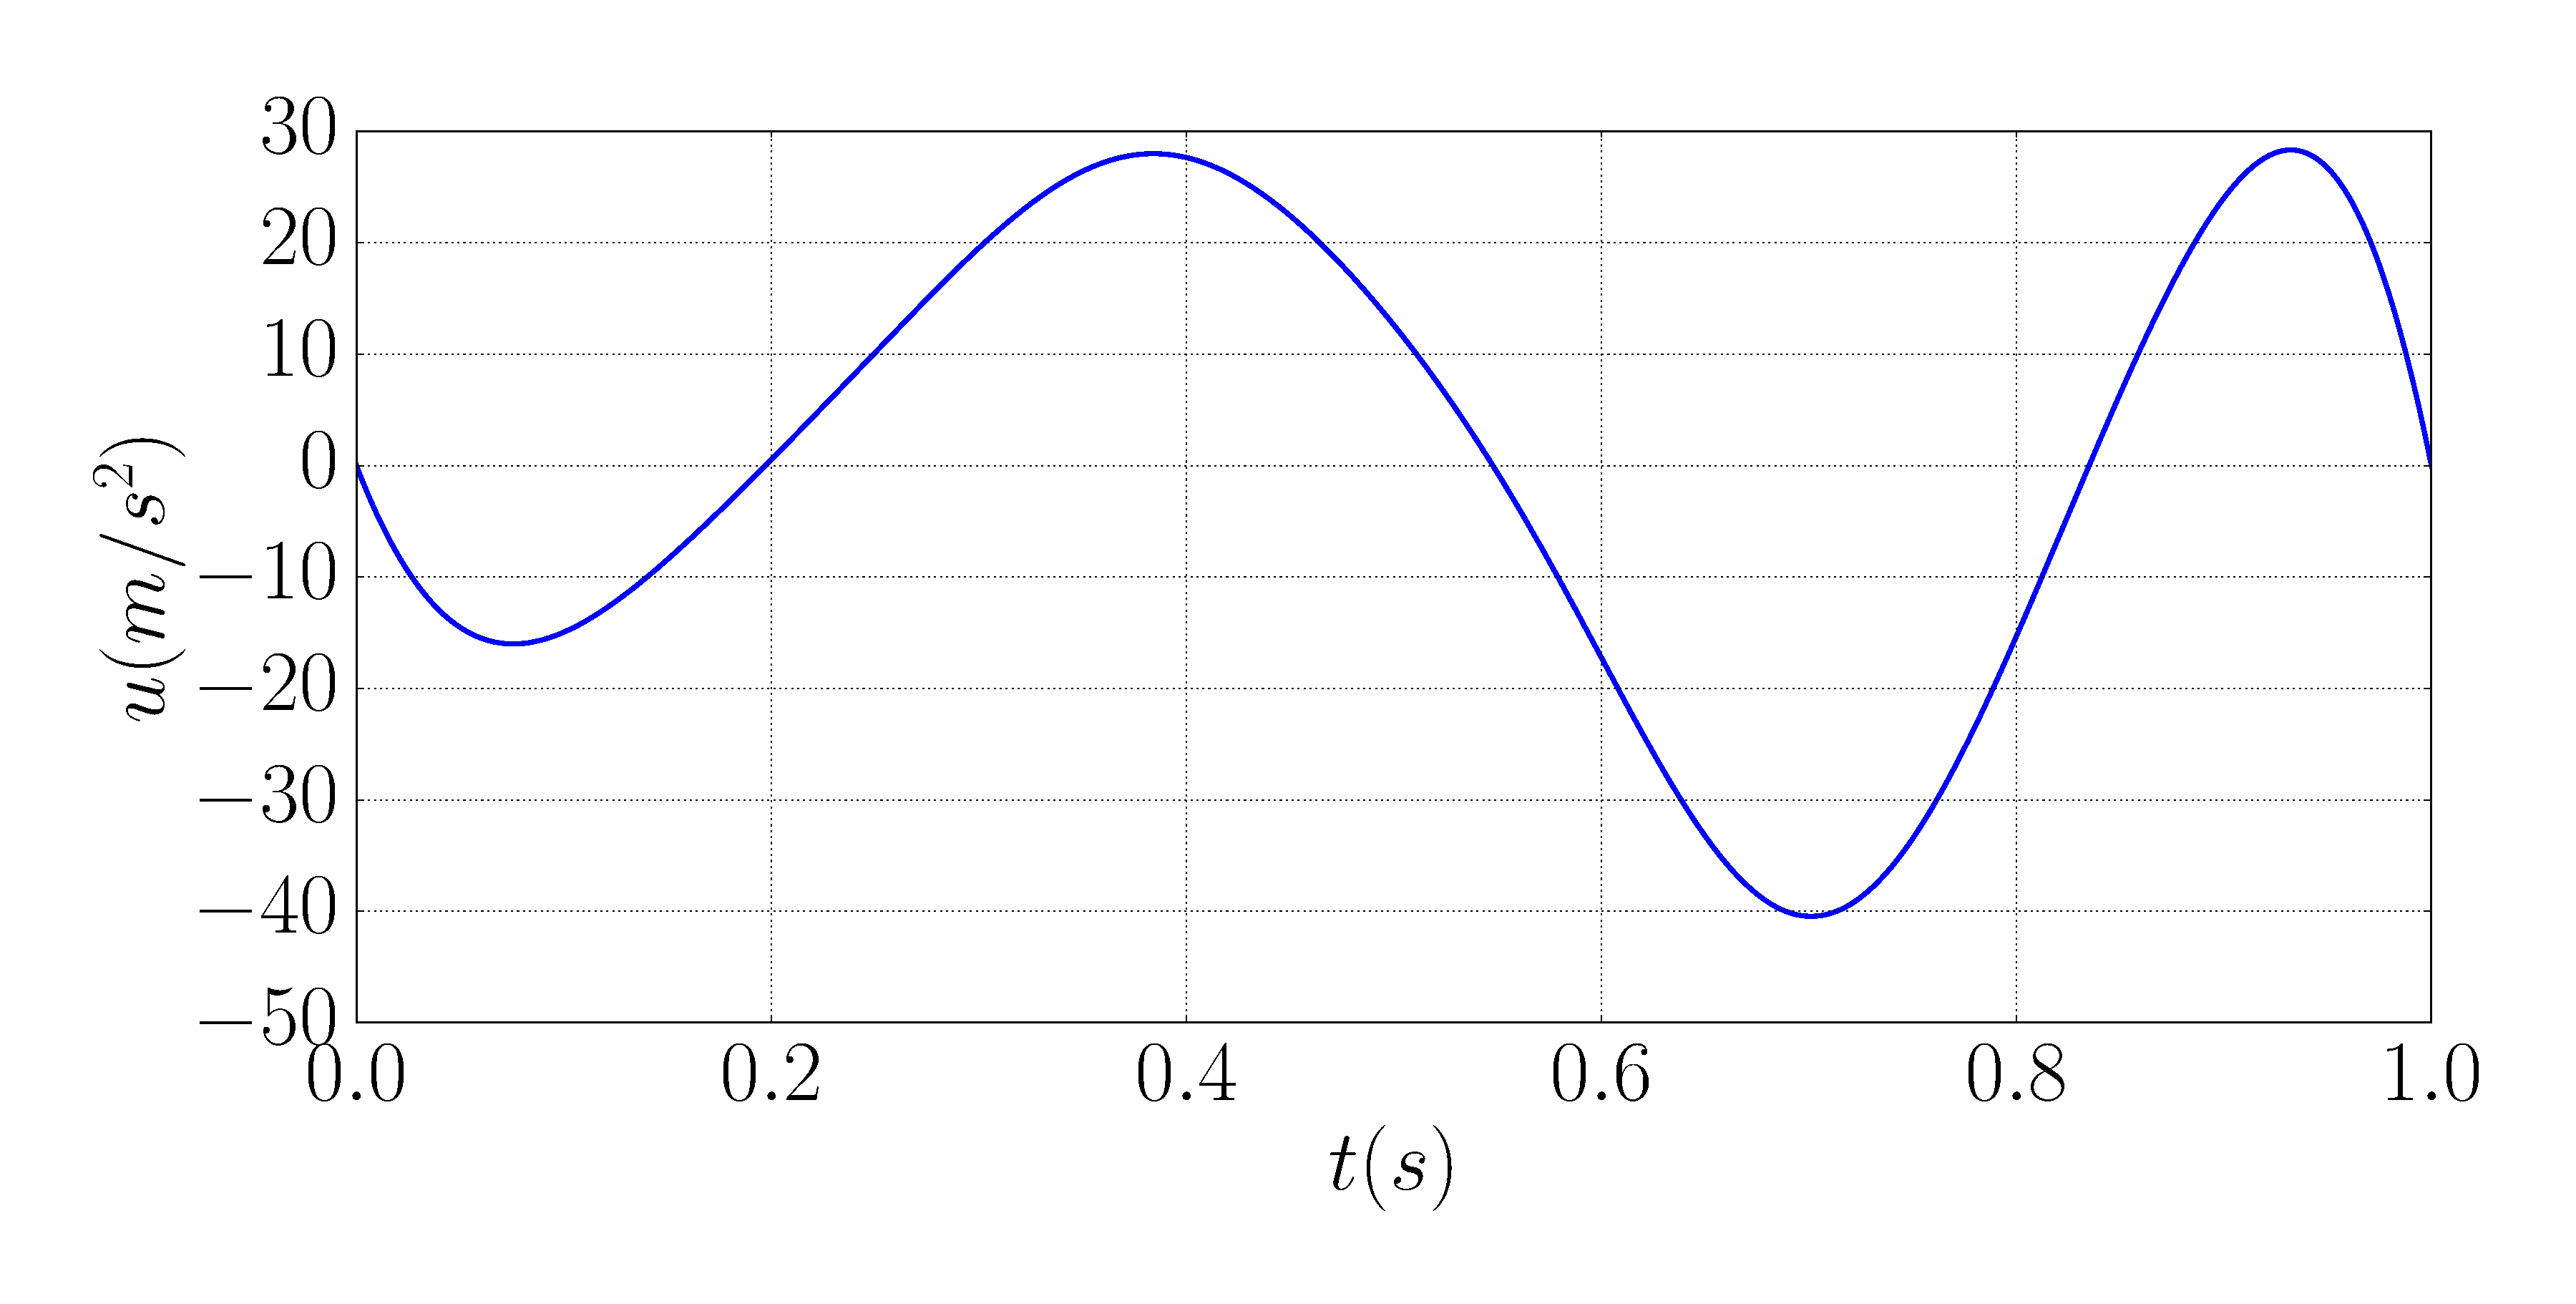
\includegraphics[width=12cm]{bild/30_32/example0_ohne_k_u.pdf}
		\caption{Systemeingang des inversen-Pendels (ohne k) mit dem virtuellen Eingang.}
		\label{fig:Inverses_Pendel_ohne_k_u}
	\end{figure}

	\begin{figure}
		\centering
		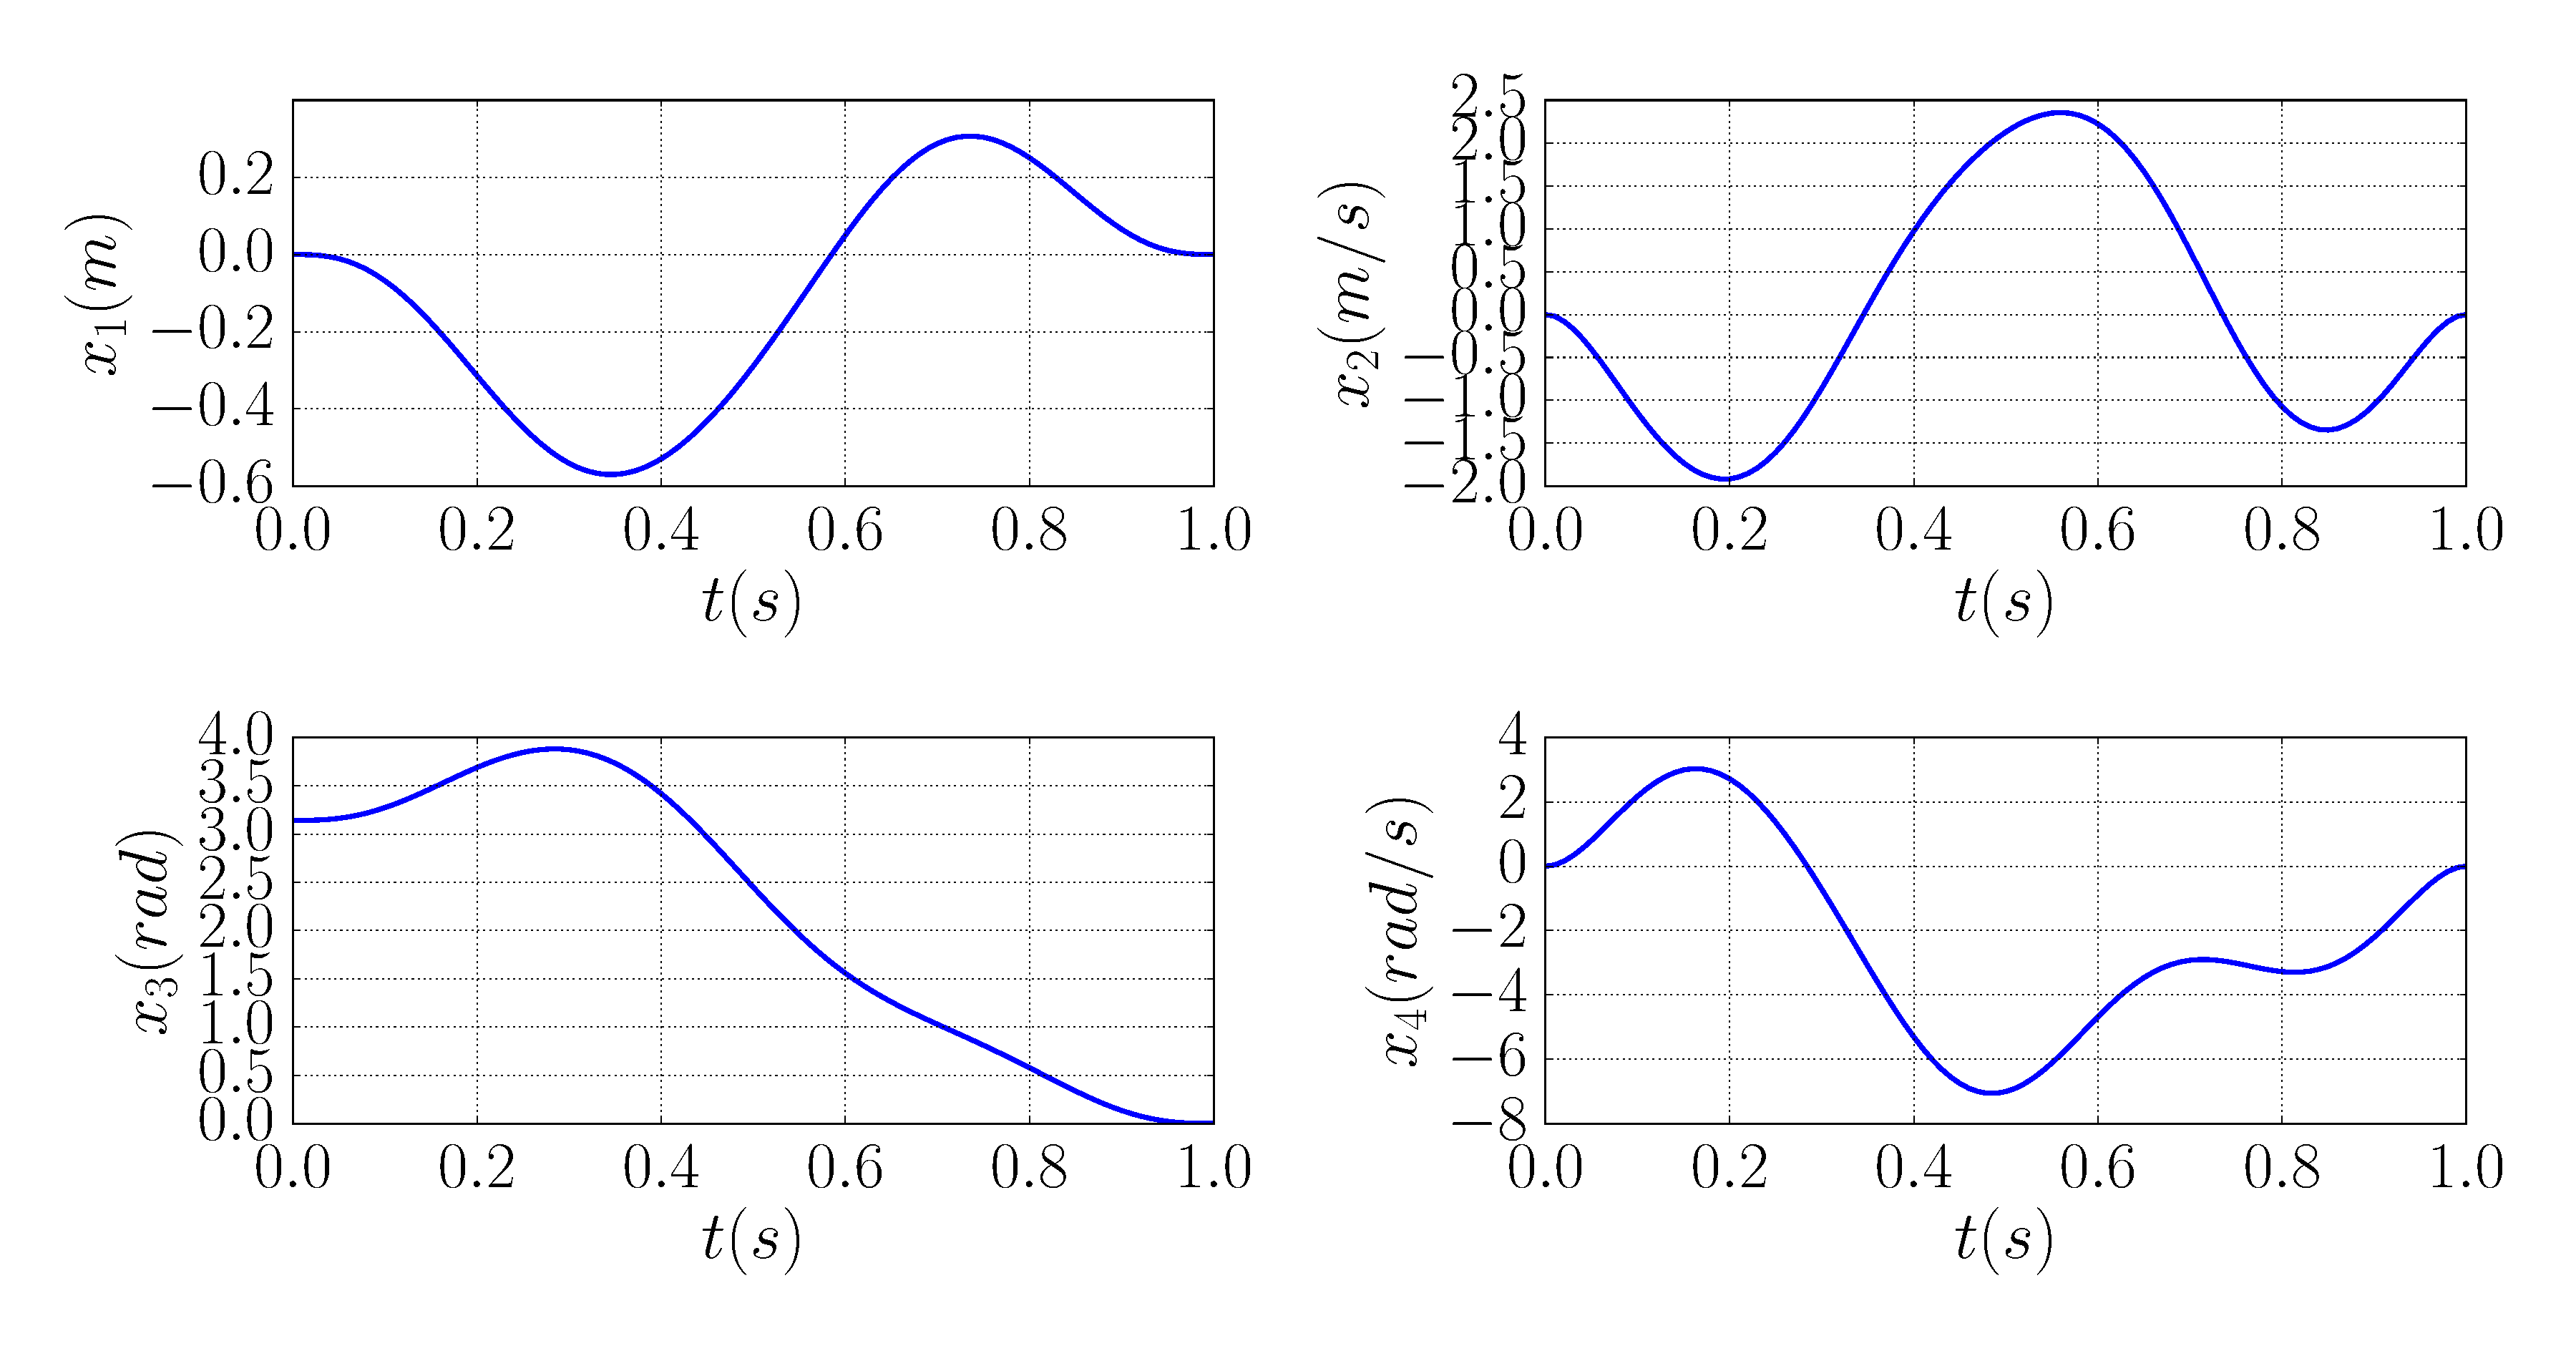
\includegraphics[width=15.5cm]{bild/30_32/example0_mit_k_x_ori.pdf}
		\caption{Systemzustandskurven des inversen-Pendels (mit k) mit dem virtuellen Eingang.}
		\label{fig:Inverses_Pendel_mit_k_x_ori}
	\end{figure}
	
	\begin{figure}
		\centering
		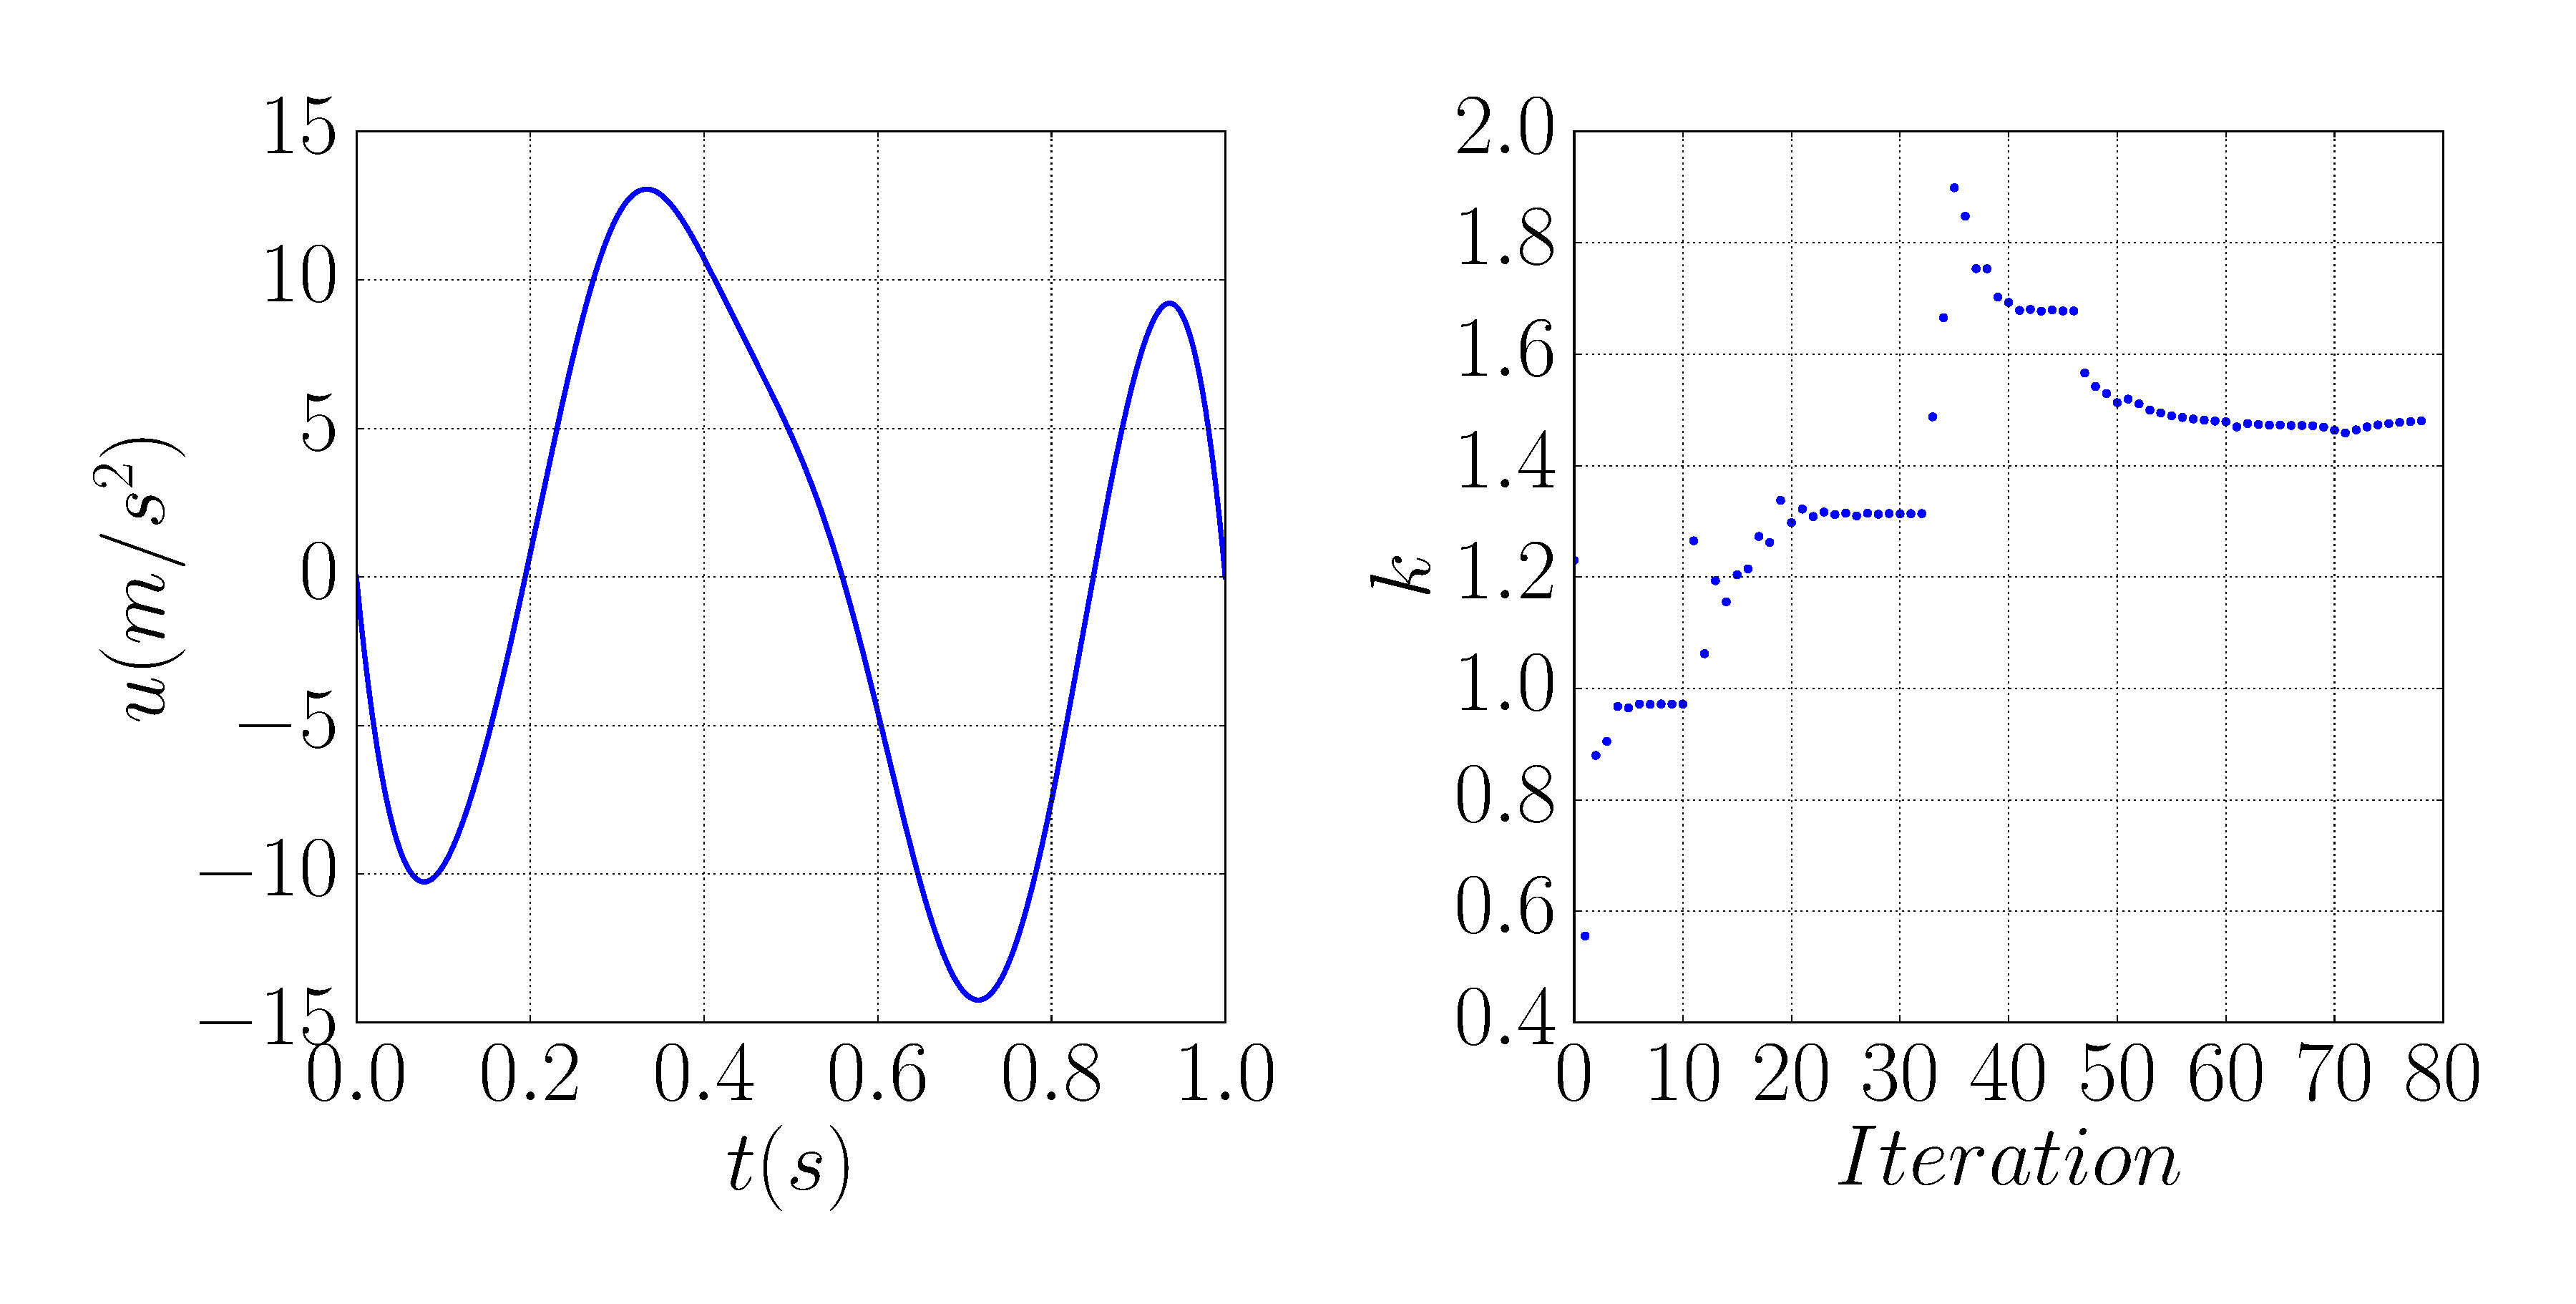
\includegraphics[width=12cm]{bild/30_32/example0_mit_k_u_ori.pdf}
		\caption{Systemeingang des inversen-Pendels (mit k) mit dem virtuellen Eingang. Die maximale Beschleunigung trägt circa $12m/s^{2}$ und nur Hälfte des Wertes in Abb. \ref{fig:Inverses_Pendel_ohne_k_u}.}
		\label{fig:Inverses_Pendel_mit_k_u_ori}
	\end{figure}
	
	Nach 5 Mal Iteration (also 32 Spline-Abschnitt) bekommen beide Systeme Lösung. Der Wert von $k$ ist $1.48$s. Egal das System ohne k oder mit k sind die Kurvenform vom Zustand und Eingang für dieses Beispiel fast gleich. Aber Offensichtlich liefert die Trajektorie des Systems mit k eine kleinere Bewegungsbereich für $\vect{x}$ und $u$ (z.B. der Bereich von $x_{1}$ ist jeweils $(0.4-+0.5)$m und $(-0.57-+0.31)$m). In Betracht auf winzigen Unterschied zwischen der Überführungszeit ist die Planung für das System mit k ausgezeichneter.
	
	Jetzt wird ein anderer Vorteil von System mit k diskutiert. Wie würde die Lösung des LM-Algorithmus verändern, wenn der Systemzustand eine Beschränkung ausgeübt würde? Der Testzustand hier ist die Wagenverschiebung $x_{1}$. Der Wagen kann nur im Bereich von $(-0.2-+0.4)$m bewegen (Die Zahl ist eine Beschränkung für beide System). Nach 8 Mal Iteration rechnet das System mit k eine Lösung mit $k=1.0535$ aus, dennoch das andere System kein Ergebnis erhalten kann (mindestens bis 8-te Iteration).
	
	\begin{figure}
		\centering
		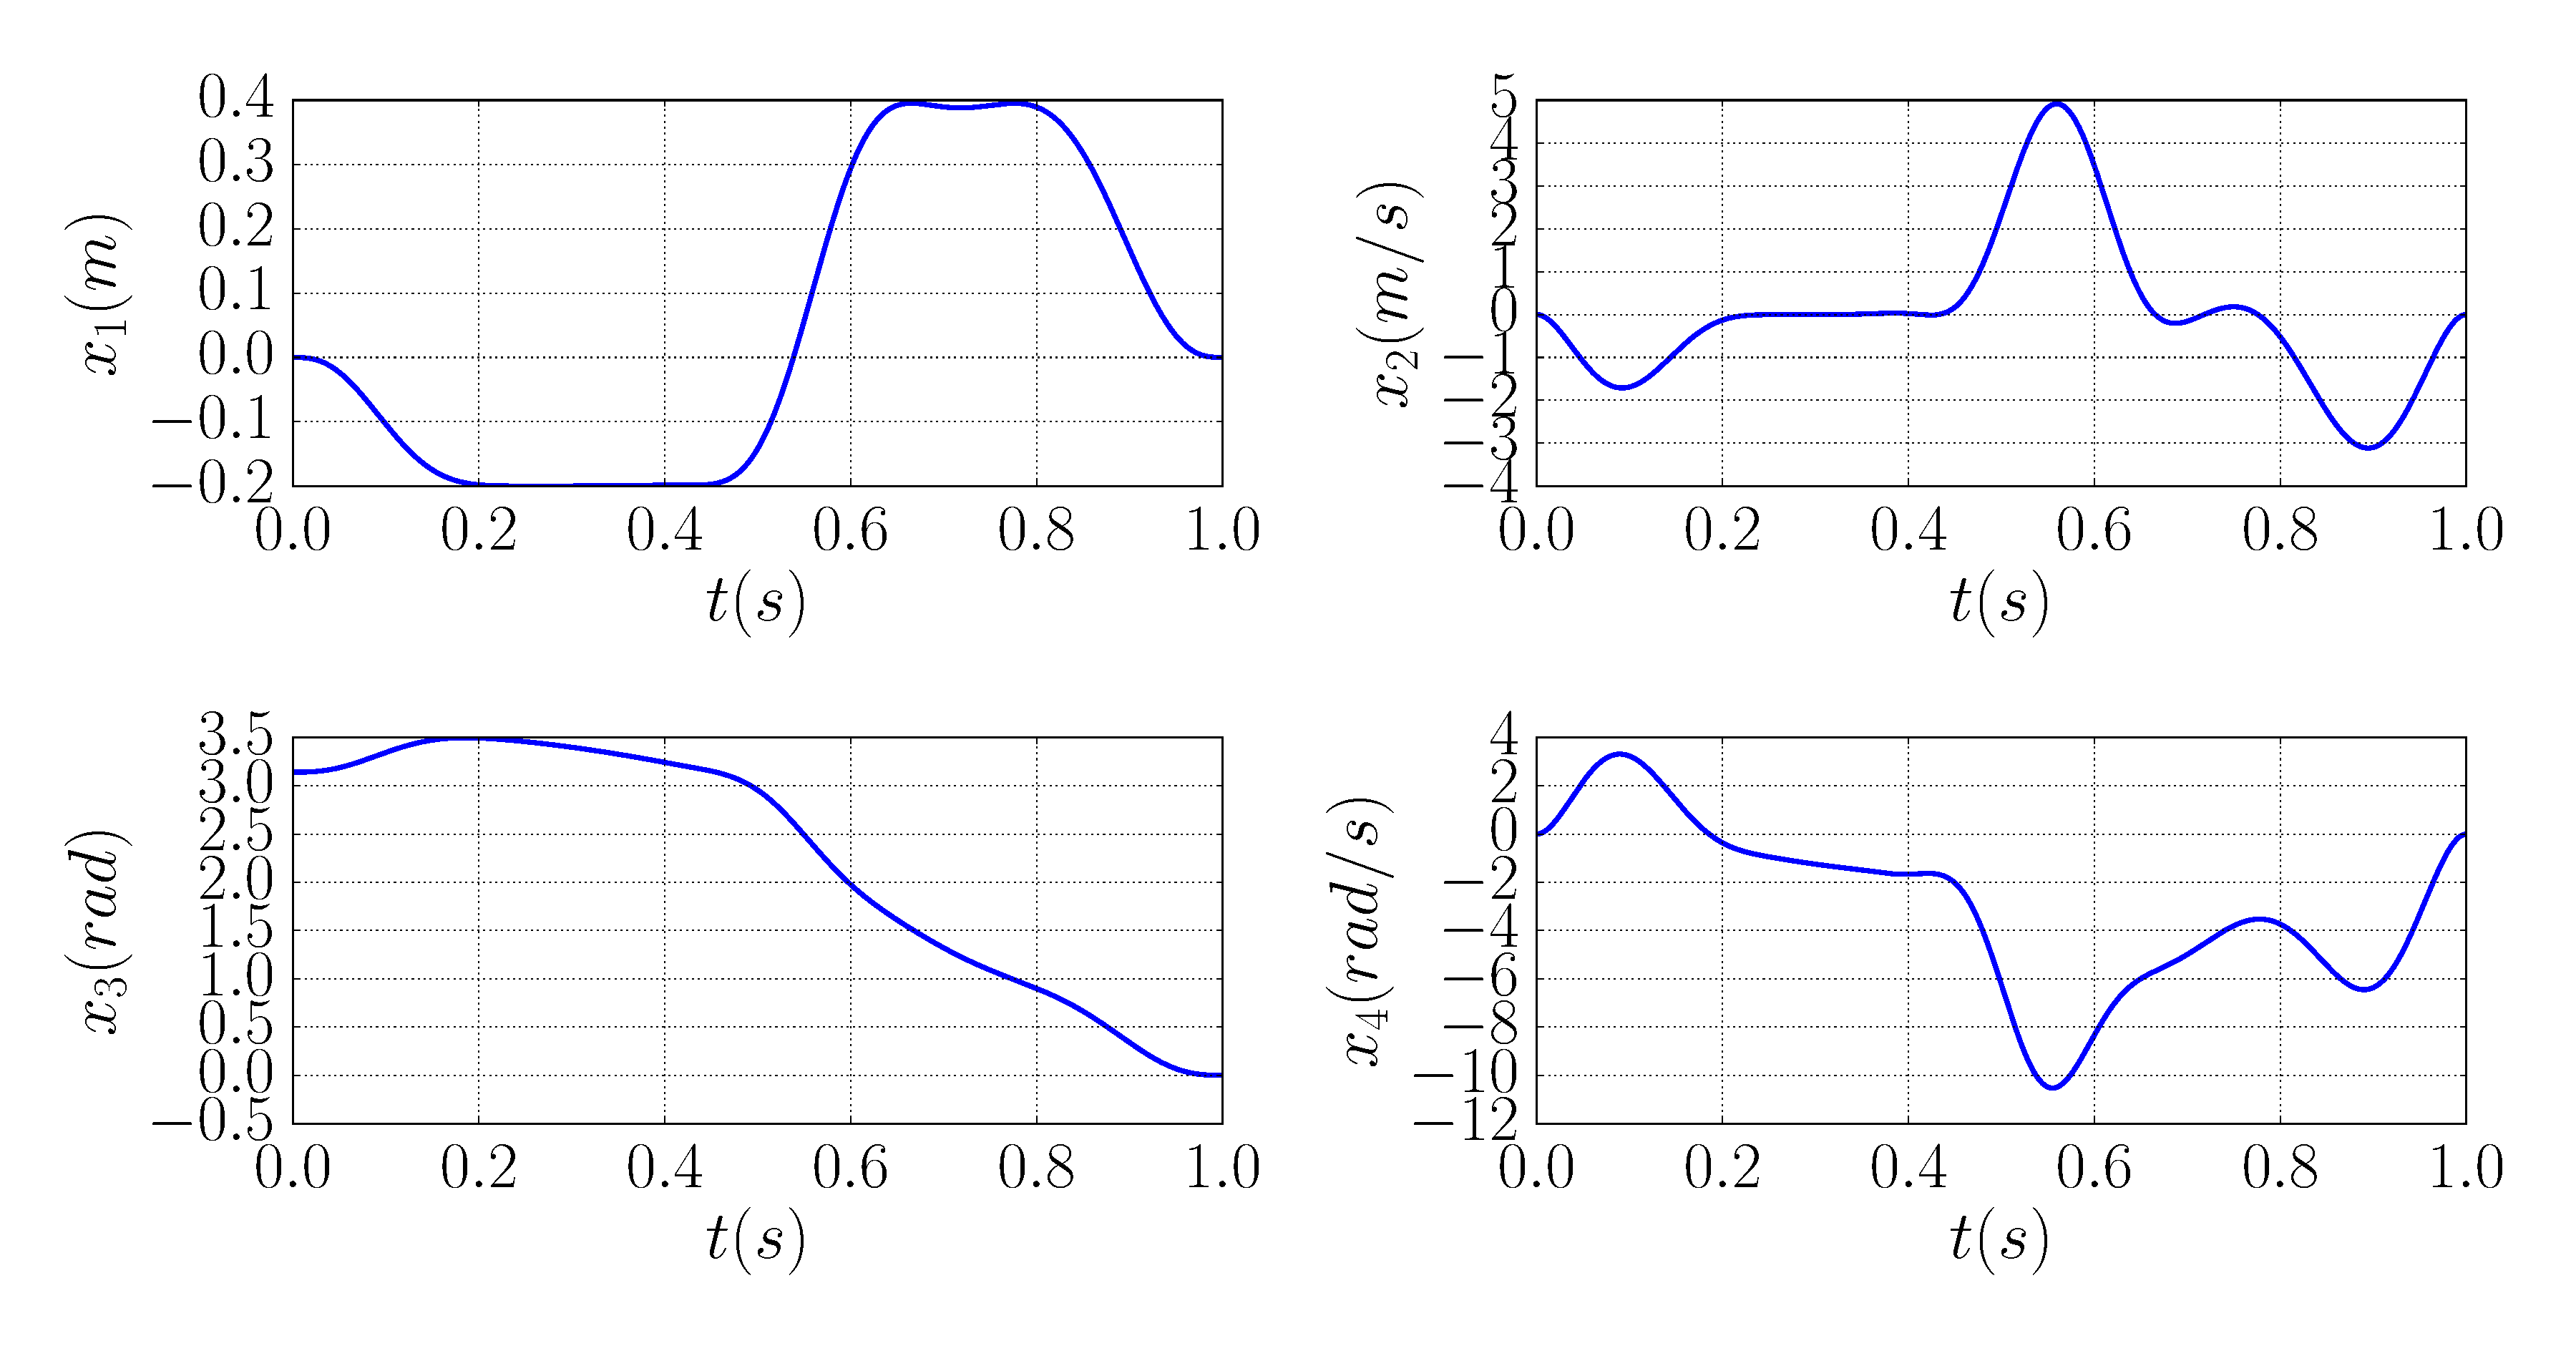
\includegraphics[width=15.5cm]{bild/30_32/example0_mit_k_x_con.pdf}
		\caption{Systemzustände des inversen-Pendels (mit k) mit dem virtuellen Eingang. $x_{1}$ ist zwischen ()$-0.2$, $0.4$) eingeschränkt.}
		\label{fig:Inverses_Pendel_mit_k_x_con}
	\end{figure}
	
	\begin{figure}
		\centering
		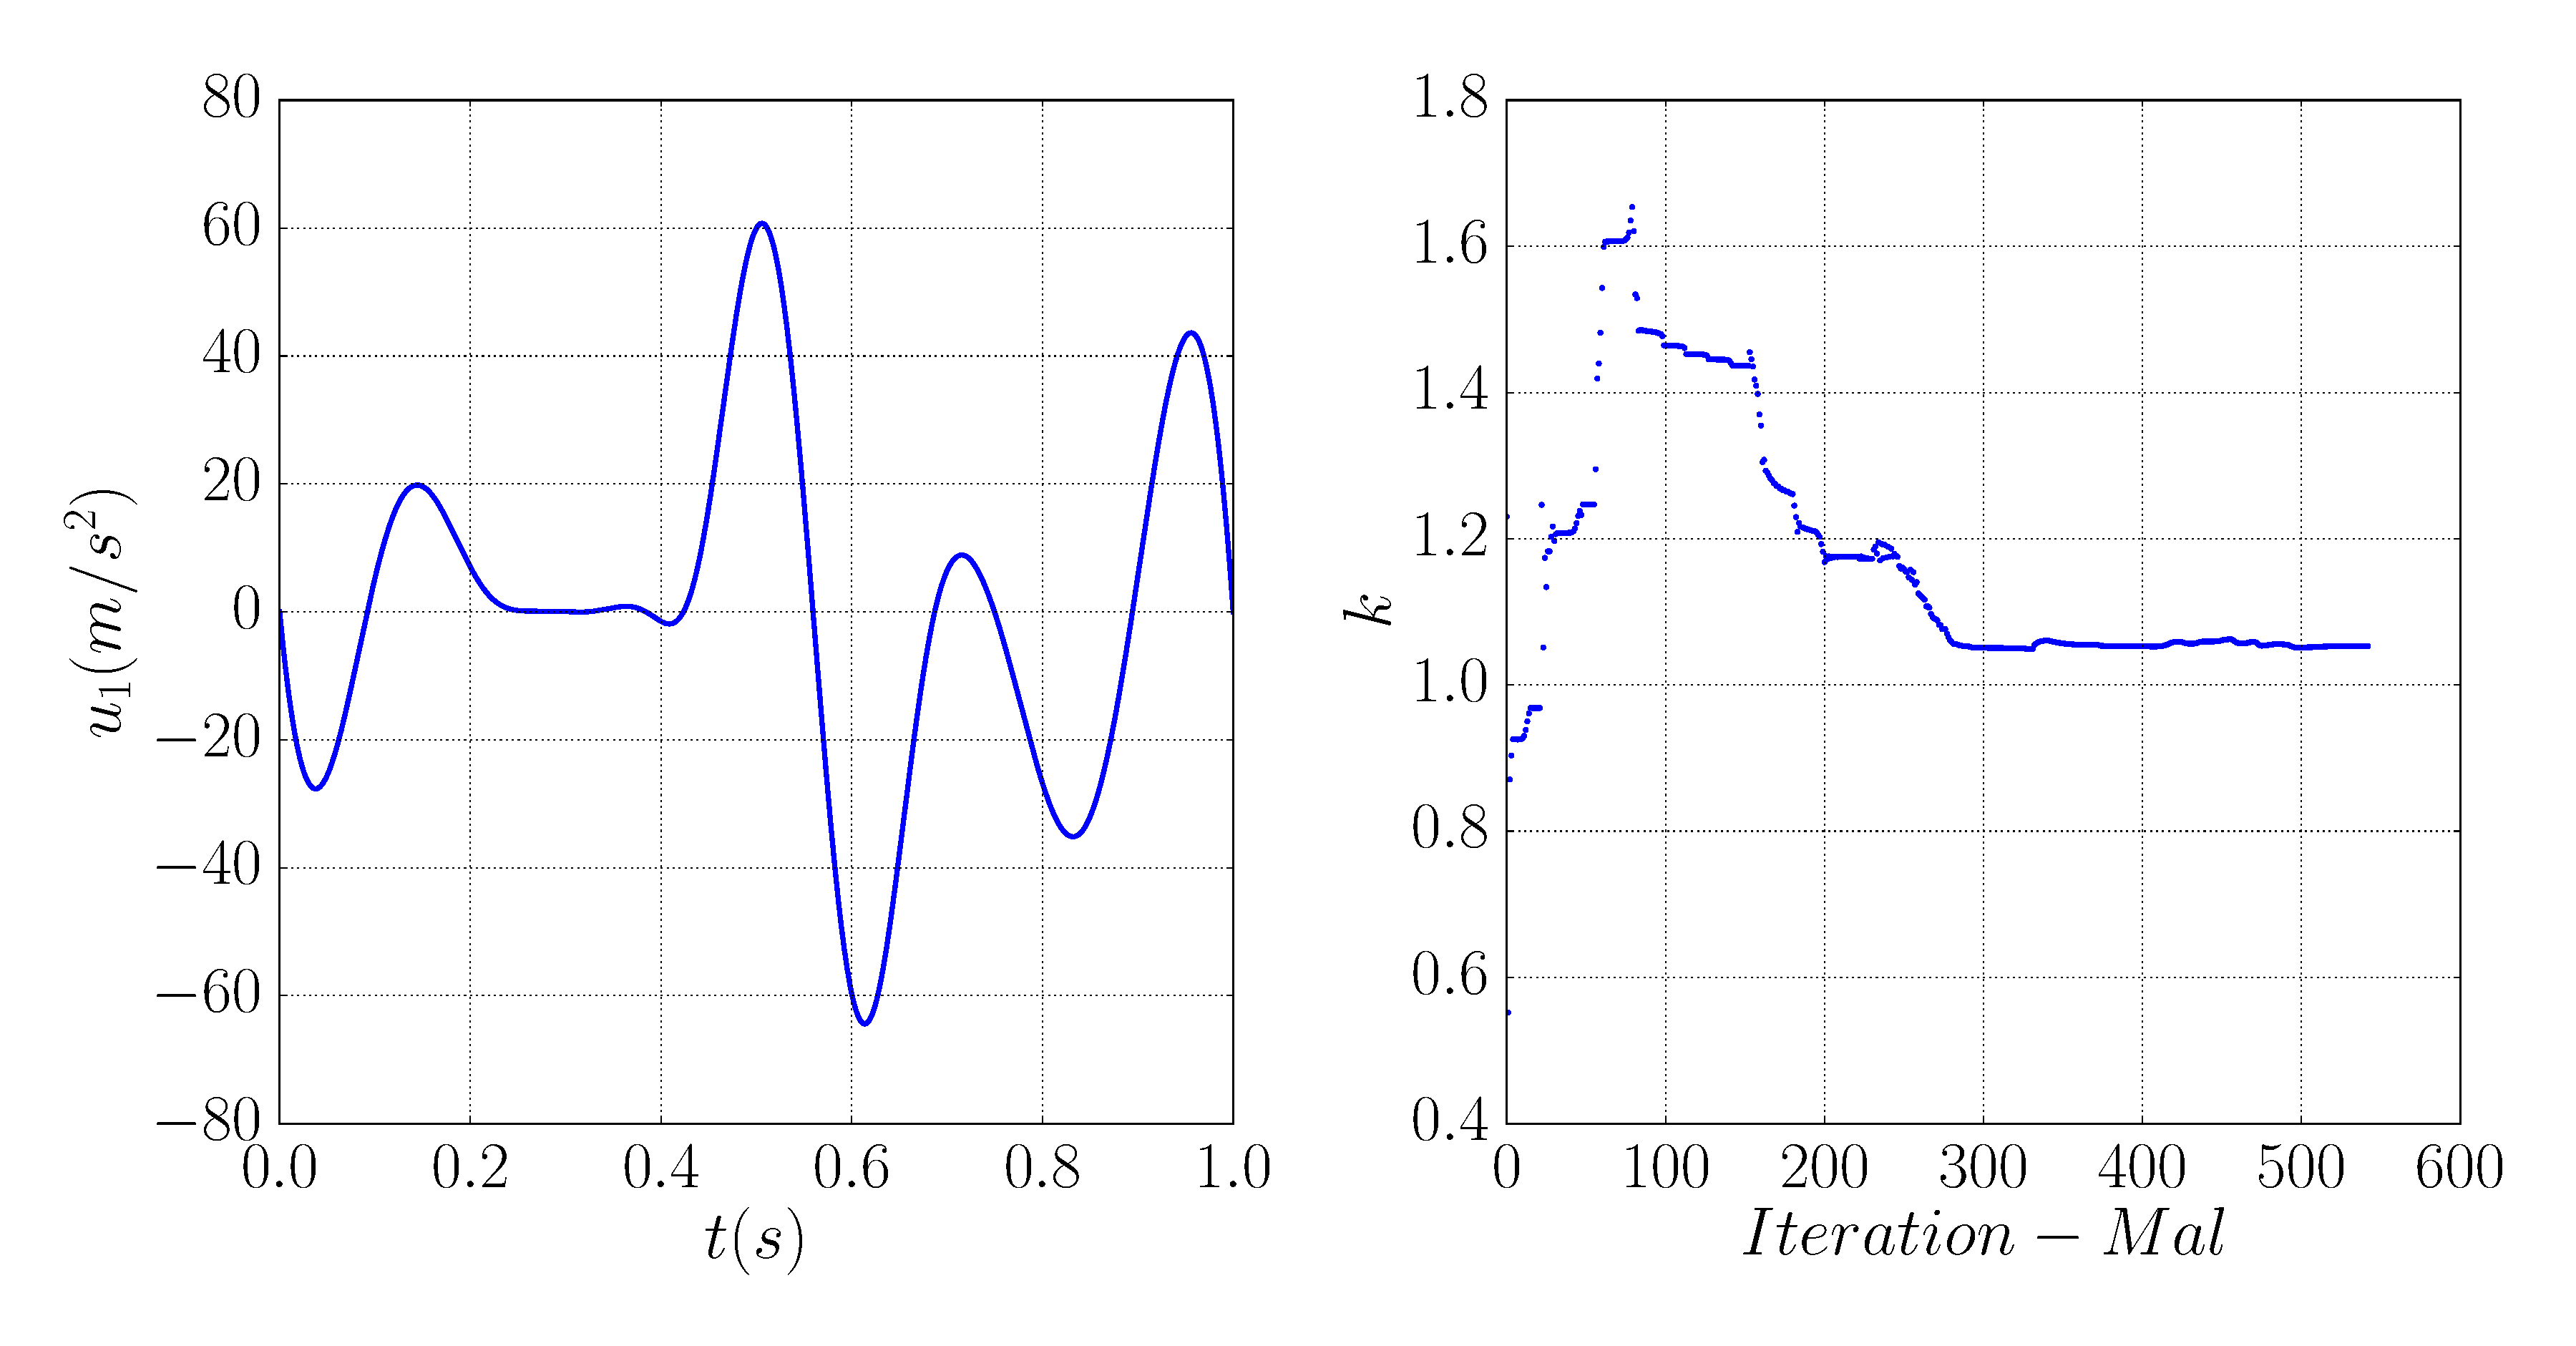
\includegraphics[width=12cm]{bild/30_32/example0_mit_k_u_con.pdf}
		\caption{Systemeingang des inversen-Pendels (mit k) mit dem virtuellen Eingang.}
		\label{fig:Inverses_Pendel_mit_k_u_con}
	\end{figure}

\end{beispiel}
\newpage
Zusammengefasst aus obere Beispiele kann das System unter Berücksichtigung der Überführungszeit eine sparsamere Trajektorie eingeplant werden, sofern gute Anfangswerte des Polynomparameter vorgegeben werden. Aber praktisch ist es nicht so einfach, einige geeignete Anfangswerte zu finden. Deswegen werden einige Methode zum Beschränken der Wertbereich von k verwendet. dass im nächsten Subschnitt beschrieben wird. % wird eine Gütefunktion von k zur Verbesserung des Überführungszeitalgorithmus entworfen, 
\subsection{Bereichgrenzung von k}
\label{Begrenzen_den_Bereich_von_k}
Die prinzipielle Idee kommt aus der Beschränkung von Systemzustände, die im Paket ``Pytrajektory'' schon realisiert wird. Der Anfangspunkt liegt in der Ersetzung der originalen Systemfunktion mit einer monotonen steigenden Sättigungsfunktion, die keine Begrenzung besitzt. Das folgt stellt die Sättigungsfunktion von ``sk'' dar.
\begin{eqnarray}
k = \psi (sk,sk^{\pm}) \notag = sk^{+}- \frac{sk^{+}-sk^{-}}{1+e^{m\cdot sk}}\label{eq:Saturation_function}
\end{eqnarray}
Weiterhin gilt $m = \frac{4}{sk^{+}-sk^{-}}$. $k$ wird in $sk^{+}$ und $sk^{-}$ beschränkt und mit der Form von $\psi$ in Systemfunktion umgeschrieben. Nachdem der Wert von $sk$ ausgerechnet wurde, wird die Lösung von $k$ auch durch Umkehrfunktion von $sk$ bekommen. Siehe \cite{graichen2006inversionsbasierter} und \cite{kunze2016pytrajectory} für weitere Information.

Das Ergebnis vom ``begrenzten $k$'' zeigt daran, den Wert von $k$ immer größer zu sein(egal ob eine approximierte Trajektorie finden kann). Aderersatz vergrößert sich $k$ zu $29.9999$ falls $sk^{+}=30$ und $sk^{-}=0.1$. Grund dafür ist die Vergrößerung der Iterationsschritt $h$ in jeder  Iteration. Wegen der unbeschränkte vergrößerte $sk$ versucht $k$ zur oberen Grenze zu erreichen.  

\subsection{Gütefunktion von k}
\label{Gütefunktion_von_k}
Eine weitere Methode zur Begrenzung von $k$ liegt darin, eine Gütefunktion am Ende der Zustandsfunktion hinzufügen. Die Gütefunktion ist eine Kombination von Parabel-und Nullfunktion. In dem von den zwei Eingänge($x_{min}$ und $x_{max}$) definierten Definitionsmenge ist die Zielmenge in der Nähe von 0. Dagegen gilt der Bildwert außerhalb diesem Bereich ähnlich wie $(x-x_{mid})^{2}$ mit $x_{mid}$ dem Mittelwert von $x_{max}$ und $x_{min}$. Die konkrete Form von \emph{pe-Funktion} ist:
\begin{eqnarray}
pe = \frac{(x-x_{mid})^{2}}{1 + e^{5\cdot (x-x_{min})}} + \frac{(x-x_{mid})^{2}}{1 + e^{5\cdot (x_{max}-x)}}\label{eq:Gütefunktion}     
\end{eqnarray}
Ein Beispiel der Kurven von \emph{pe} mit $x_{min}=0$ und $x_{max}=10$ ist wie Abb.\ref{fig:Gütefunktion_von_k} gezeigt. Zwischen $(0,10)$ ist $pe$ ungefähr 0. Der andere Teil läuft wie eine Parabel. Mit dieser Gütefunktion von $k$ probiert das System eine Lösung in der Nähe von $x_{mid}$ zu finden.
\begin{figure}
	\centering
	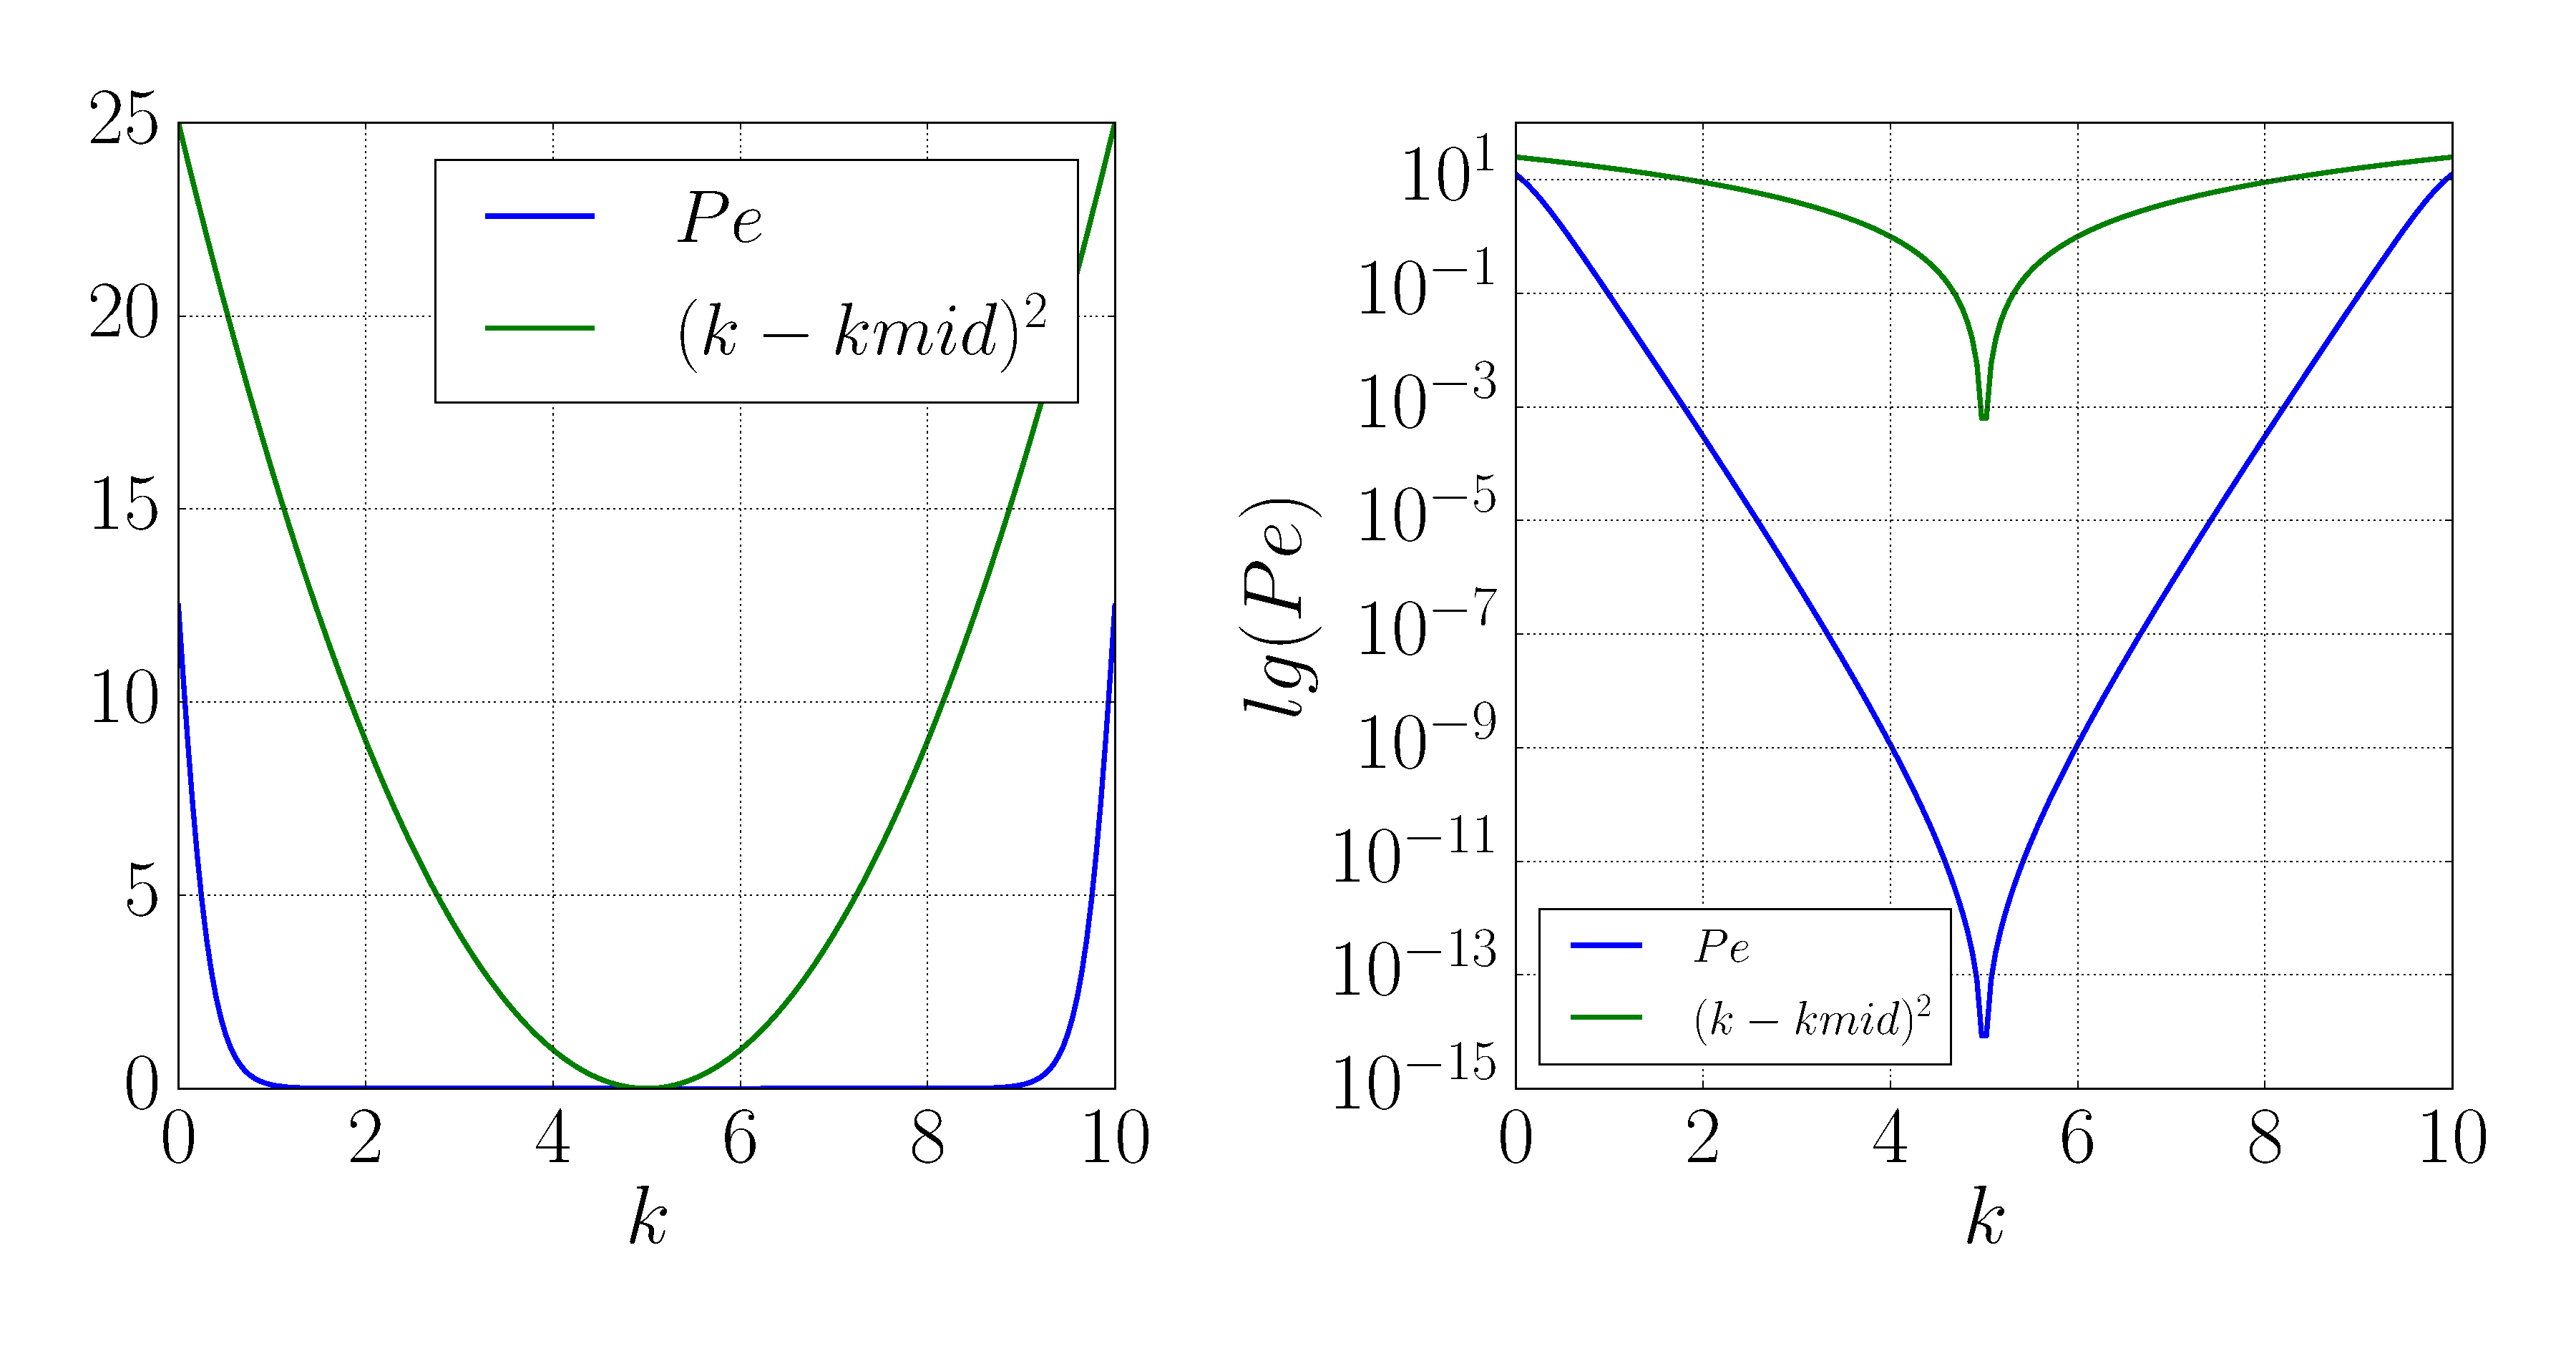
\includegraphics[width=12cm]{bild/pe/pe.pdf}
	\caption{Gütefunktion von k: $x_{min}=0$, $x_{max}=10$}
	\label{fig:Gütefunktion_von_k}
\end{figure}
\begin{beispiel}
	Geht man zurück auf das Beispiel Doppelintegrator. Angenommen, dass $x_{min}$ und $x_{max}$ jeweils $0.1$, $3$ und der Anfangsschätzwert von $k$ $1.5$ ist. Die andere Bedingungen bleiben wie zuvor.
	Die Zeitverlauf vom Eingang $u$ ist noch sinusförmig aber mit dem maximalen Wert $4m/s^{2}$. Der maximale Wert von der Wagengeschwindigkeit $x_{2}$ ist auch ähnlich wie das System ohne $k$: circa $1.6m/s$. In Anbetracht auf das Ergebnis und die Lösung von $k$ ($1.87$) zeigt dieses Beispiel eine annähernde Trajektorie wie das originale System. 
\end{beispiel}


